\documentclass[a4paper]{book}

%PACKAGES
\usepackage[T1]{fontenc}
\usepackage[utf8]{inputenc}
\usepackage[italian]{babel}
\usepackage{amsfonts} 
\usepackage{amssymb} 
\usepackage{amsmath}
\usepackage{amsthm}		%teoremi
\usepackage{graphicx}	%immagini
\usepackage{setspace}	%interlinea
\usepackage{tikz}		%disegnare immagini
\onehalfspacing


%THEOREMS, ...
\theoremstyle{definition}
\newtheorem{ex}{Esempio}
\newtheorem{defn}{Definizione}

\theoremstyle{remark}
\newtheorem{oss}{Osservazione}
\newtheorem{dimst}{Dimostrazione}
\newtheorem{idea}{Idea}

\theoremstyle{definition}
\newtheorem{lem}{Lemma}
\newtheorem{teo}{Teorema}
\newtheorem{prop}{Proprietà}
\newtheorem{coroll}{Corollario}


%NEW COMMANDS
\newcommand{\bbx}{\mathbb{X}}
\newcommand{\bbr}{\mathbb{R}}
\newcommand{\bbn}{\mathbb{N}}
\newcommand{\ra}{\Rightarrow}
\newcommand{\vp}{\varphi}

\title{Calcolo delle variazioni \\ \small{Lezioni di Gobbino 17/18} }
\author{}

\begin{document}

\maketitle
\chapter{Lezione 1}
Il calcolo delle variazioni consiste nello studio di problemi di minimo.
\\
In particolar modo, abbiamo un insieme $\bbx$ ed una funzione $f:\bbx \to \bbr$ e vogliamo trovare min$\{f(x)|x \in \bbx\}$.
\\
Ci sono 4 metodi di approccio al problema:
\\
1.\textbf{Metodo indiretto}	\hspace{3mm}2.\textbf{Metodo diretto} \\
3.\textbf{Rilassamento}	\hspace{3mm}	4.\textbf{Gamma-convergenza}

\begin{ex}
\[
	f:\bbr \to \bbr, f = x^2 - 4x
\]
\[
	\textsf{Metodo indiretto: }f'(x) = 2x - 4 \ra f'(x) = 0 \iff x = 2 \ra \textit{min} = f(2) = -4
\]
Proviamo adesso a dimostrare che $f(x)$ è sempre $\leq$ di $-4$ \footnote{Questa è la vera dimostrazione}.
\[
	x^2 - 4x \ge -4 \iff x^2 -4x + 4 \ge 0 \iff (x -2)^2 \ge 0 
\]
che è vero, inoltre vale l'uguaglianza se e solo se $x = 2$. \\
Metodo diretto: dimostriamo che il minimo esiste, ad esempio usando il teorema di Weierstrass generalizzato:
\[
	f: \bbr \to \bbr \textit{ continua e } \lim_{x \to \pm\infty}f(x) = \infty \ra \textit{il minimo esiste}
\]
Ora che so che esiste posso vedere dove $f'(x) = 0$.
\end{ex}

\begin{ex}
	Cerchiamo min$\{(x^2 - 2)^2 | x \in \mathbb{Q} \}$ \\
	In questo caso il minimo non esiste. Possiamo perciò chiederci: chi è l'inf? Come sono fatte le successioni "minimizzanti"?\\
	L'inf è 0 e le succ. min. hanno una sottosuccessione che tende a $\pm \sqrt 2$.
\end{ex}
\noindent
\textbf{Rilassamento}: Con questo metodo rilassiamo le condizioni imposte dal problema e per farlo possiamo procedere in due modi:
1.Estendo f ad un ambiente più vasto; \\
2.Cambio la funzione in modo che il minimo abbia più probabilità di esistere.	

\begin{ex}
Consideriamo una famiglia di problemi di minimo:
\[
	m_n := min\{e^{x^2} + atg(x) + nsin^2(x)|x \in \bbr^n \}
\]
e chiediamoci:\\
a cosa tende $m_n$ quando $n \to\infty$?\\
a cosa tendono i punti di minimo quando $n \to\infty$?\\
Ci aspettiamo che $m_n \to m_{\infty} := min\{e^{x^2} + atg(x) | x = k\pi, k \in \mathbb{Z} \}$\\
Per rispondere a queste domande usiamo la gamma convergenza.
\end{ex}

\begin{defn}
Generalemente $\bbx$ sarà uno spazio di funzioni. Chiameremo allora 
\[
 	F :\bbx \to \bbr 
 \] 
\textbf{Funzionale}
\end{defn}

\begin{ex}
\[
	F(u) = \int_2^4 (\dot u^2 + sin(u))\,dx
\]
\end{ex}
\noindent
Un particolare tipo di funzionali sono poi quelli $\textbf{integrali}$
\[
	F(u) := \int_a^b L(x, u(x), \dot u(x))\,dx
\]
con $L: [a,b]\times\bbr\times\bbr \to \bbr$.\\
In generale scriveremo $L(x, s, p)$ dette Lagrangiane.\\
Altre generalizzazioni possibili sono:
\[
	F(u) := \int_{a}^{b} L(x, u, \dot u, \ddot u, \dots)dx
\]
\[
	F(u, v) := \int_a^b L(x, u, v, \dot u, \dot v, \dots)dx
\]

\begin{oss}
Problemi più complicati sono del tipo:\\
1.Più variabili in partenza\\
2.Più variabili in partenza e arrivo (caso vettoriale)
\end{oss}

\begin{ex}[Classico]
Data f(x) trovare\\
\[
	min\{\int_a^b \dot u^2 + (u - f)^2\,dx | u \in C^1([a,b])\}
\]

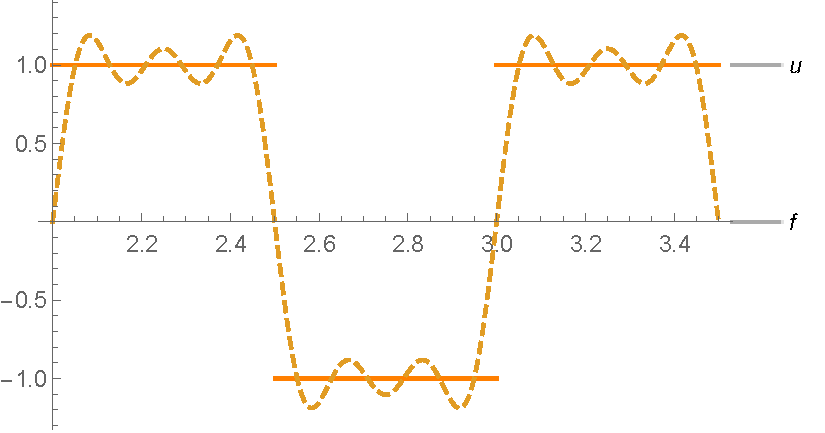
\includegraphics[scale = 0.5]{Fourier_onda_quadra.pdf}\\
\noindent
con f che può essere ad esempio il segnale di un cellulare.
\end{ex}

\begin{ex}[Classico]
\[
	min\{\int_a^b(\dot u^2 + u)dx | u(a) = A, u(b) = B, u \in C^1([a,b])\}
\]
con A e B dati\\
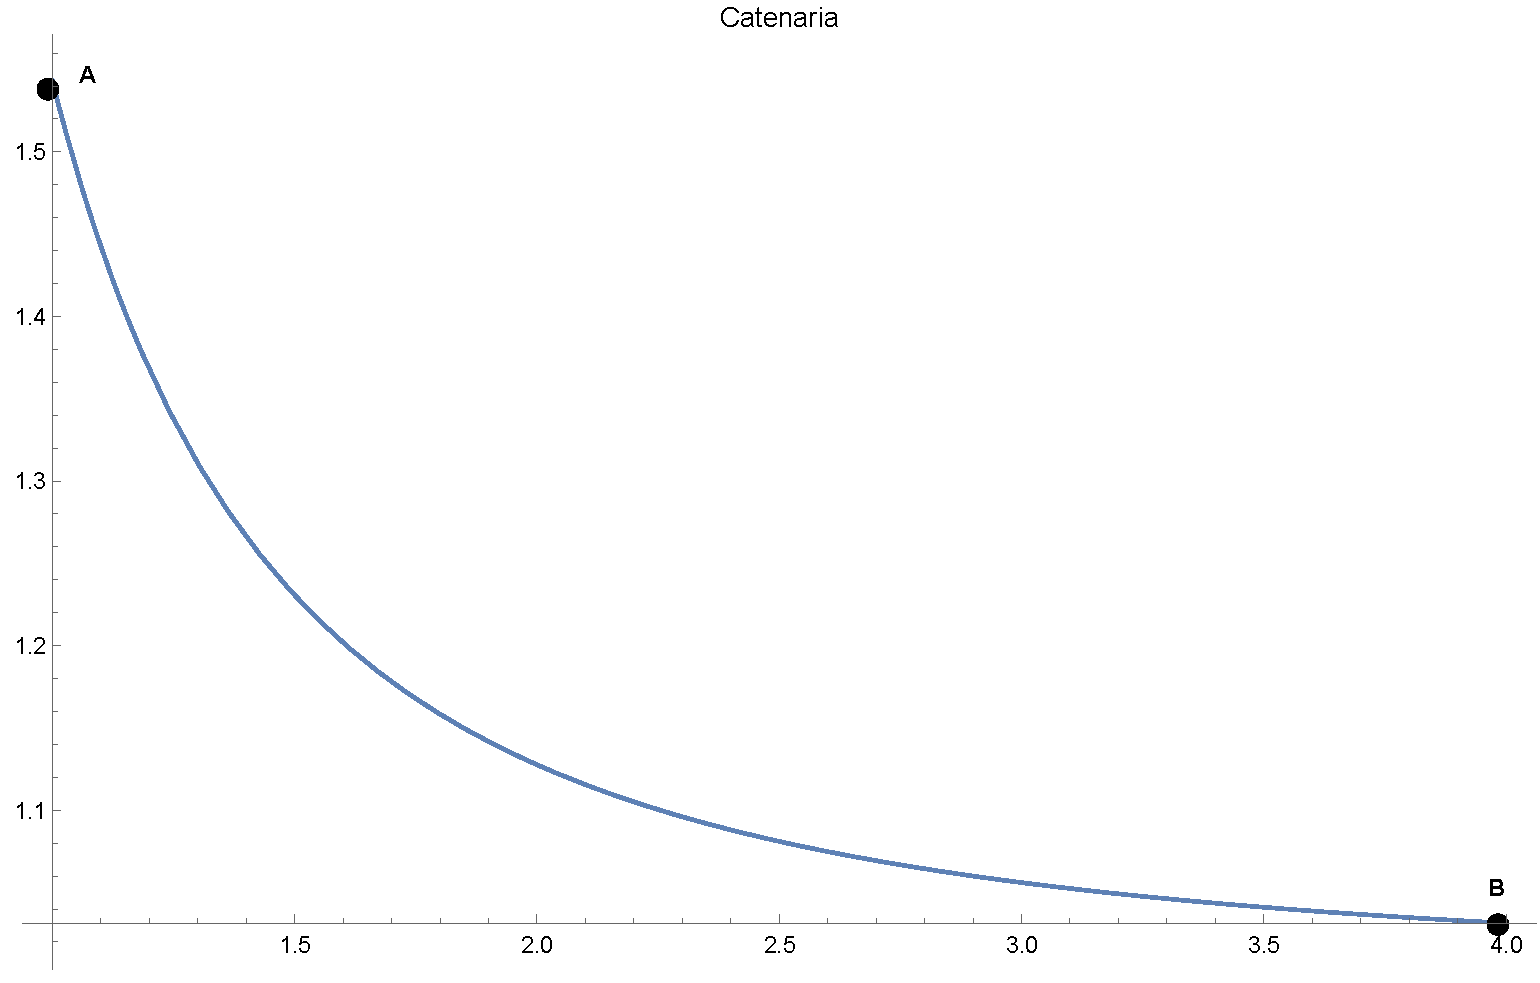
\includegraphics[scale = 0.4]{catenaria.pdf}
\end{ex}

\chapter{Lezione 2}
La variazione prima di un funzionale è l'analogo della derivata prima per una funzione.
\begin{defn}
Consideriamo un insieme $\bbx$ ed $f:\bbx \to \bbr$. Sia $x_0$ un punto di minimo e siano $\delta > 0, \gamma:(-\delta, \delta)\to \bbx$ t.c. $\gamma(0)=x_0$.
Posso considerare la funzione composta
\[
	\varphi(t) := F(\gamma(t)) \in \bbr
\]
Allora
\[
	\varphi:(-\delta, \delta)\to\bbr
\]
con minimo in t=0.\\
Pongo allora $\delta F(x_0, \gamma):=\varphi'(0)$(\footnote{Posto che esista}).\\
$\delta F(x_0, \gamma)$ è detto \textbf{Variazione prima del funzionale F lungo una curva $\gamma$}.
\end{defn}

\begin{oss}
La definizione è valida $\forall x_0$, anche non di minimo, e $\forall$ curva $\gamma : \gamma(0) = x_0$ purchè $\varphi'(0)$ esista.
\end{oss}

\begin{lem}
Se $x_0 \in argmin\footnote{$x \in \bbx$ t.c. f(x) è un minimo} \{f(x)|x\in\bbx \}$, allora 
\[
	\delta F(x_0, \gamma) = 0
\]
quando esiste.
\end{lem}
\noindent 
Supponiamo ora che $\bbx$ sia uno spazio affine con spazio vettoriale di riferimento\footnote{traslato che passa per l'origine, detto anche giacitura} V.\\
In particolare
\[
	\forall u \in \bbx, \forall v \in V \textit{ si ha che } u + v \in \bbx
\]
In questo caso, dati $u_0 \in \bbx$ e $v \in V \smallsetminus \{ 0 \}$ posso considerare la curva
\[
	t \to u_0 + tv : \textit{retta per $u_0$ con direzione v}
\]
e calcolare
\[
	\delta F(u_0, v) := \footnote{"derivata direzionale" o "alla Gateaux"} \lim_{t \to 0} \frac{F(u_0 + tv) - F(u_0)}{t}
\]

\begin{ex}
Consideriamo 3 funzionali
\[
	F(u) = \int_a^b \dot u^2(x)dx \qquad G(u) = \int_a^b |\dot u(x)|dx \qquad H(u) = \int_a^b \sqrt{|\dot u(x)|}dx
\]
con $\bbx = \{u\in C^1([a,b]) | u(a) = A, u(b) = B \}$ 


\begin{oss}
$\bbx$ è uno spazio affine con giacitura
\[
	V = \{v \in C^1([a,b])| v(a) = v(b) = 0\}
\]
\end{oss}
\noindent 
\textit{Metodo indiretto:}
\[
	\varphi(t) = F (u + tv) = \int_a^b(\dot u + t \dot v)^2\,dx = \int_a^b \dot u^2 + \int_a^b 2t\dot u \dot v + \int_a^b t^2 \dot v^2
\]
\[
	\ra \delta F(u, v) := \varphi'(0) \stackrel{\footnote{Deriviamo rispetto a t}}{=}  2\int_a^b \dot u \dot v 
\]
Questa è detta \textbf{Prima forma integrale della variazione prima}.\\
Integriamo adesso per parti:
\[
	\varphi'(0) = 2[\dot u v]_a^b - 2 \int_a^b \ddot u v = \underbrace{2(u(b)v(b)-u(a)v(a))}_{0} - 2\int_a^b \ddot u v = -2\int_a^b \ddot u v
\]
Questa, invece, è detta \textbf{Seconda forma integrale della variazione prima}.

\begin{oss}
Abbiamo usato $\ddot u$ che non è detto esista, ma tanto siamo ancora nella parte preliminare e non devo necessariamente essere formale.
\end{oss}
Allora se $u_0$ è un punto di minimo 
\[
	\int_a^b \dot u_0 \dot v = 0 \qquad \forall v \in V
\]
e se u fosse $C^2$
\[
	\int_a^b \ddot u_0 v = 0 \qquad \forall v \in V
\]
Dalla seconda sembra ragionevole dedurre che 
\[
	\ddot u_0(x) \equiv 0 \ra u_0(x) =\textit{retta } A \to B
\]
Forniamo adesso la dimostrazione rigorosa:\\
Sia $u_0(x)$ la retta e sia $w(x)$ un qualunque altro elemento di $\bbx$. Allora 
\[
	v = w - u_0 \in V
\]
quindi si annulla in a e b.
\[
	F(w) = F(u_0 + v) = \int_a^b (\dot u_0 + \dot v)^2 = \underbrace{\int_a^b \dot u_0^2}_{F(u_0)} + \underbrace{2\int_a^b \dot u_0 \dot v}_{0 \footnote{Integrando per parti poichè $u \in C^2$}} + \underbrace{\int_a^b \dot v ^2}_{\ge 0} \ge F(u_0) \qquad w(x)
\]
Abbiamo così dimostrato che $F(w) \ge F(u_0)$ e vale l'uguale $\iff \int_a^b \dot v^2 = 0\iff\dot v(x) = 0 \iff v(x) = c.te$, ma $v(a)=v(b)=0 \ra v(x)=0 \ra w(x)  u_0(x)$.\\
Quindi la retta è l'unico punto di minimo 
\[
	\ddot u_0(x) = 0 \qquad \forall x \in [a,b]
\]
Quest'ultima equazione è detta \textbf{Forma differenziale di ELE} \footnote{Equazioni di Eulero-Lagrange}.\\

Passiamo adesso al funzionale H.\\
Dico che $infH = 0$ e non è minimo a meno del caso banale A = B.\\
Infatti
\[
	H(u_n)=\int_{b-1/n}^b |\dot u_n(x)|^2\,dx = \int_{b-1/n}^b |(B-A)n|^{1/2}\,dx = |B-A|^{1/2}\sqrt n \frac1n \to 0 \qquad \textit{per } n \to \infty
\]	
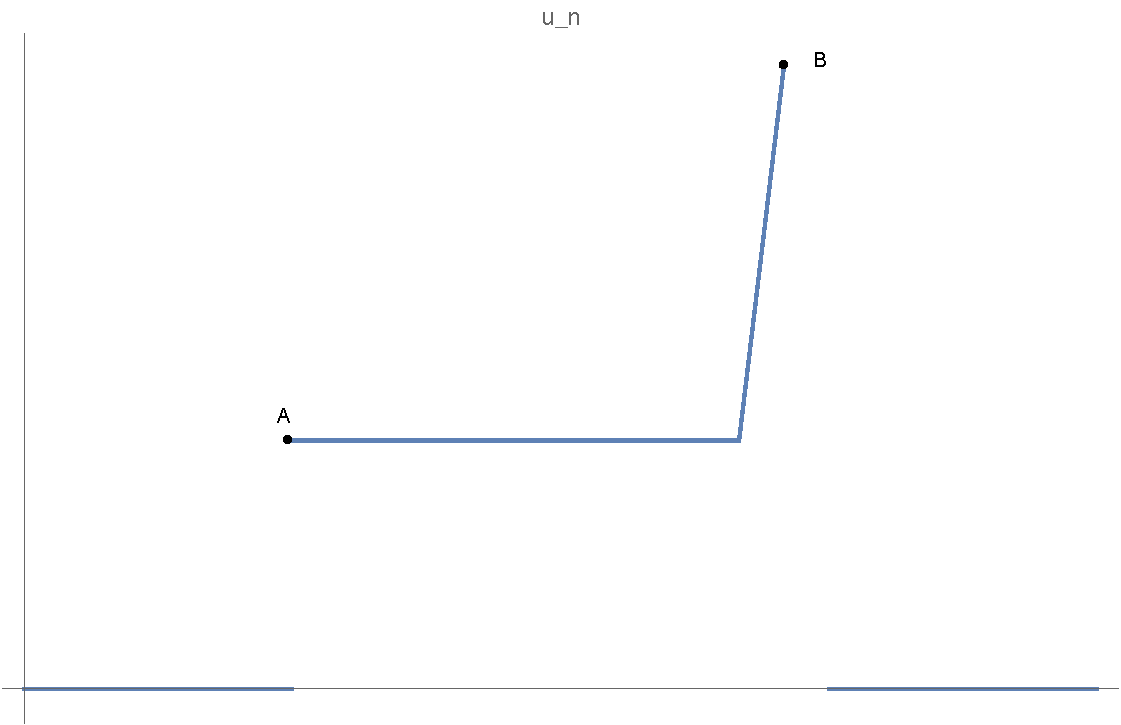
\includegraphics[scale=0.4]{u-n.pdf}

\begin{oss}
Non sarebbe $C^1$, ma fare un piccolo raccordo derivabile conta davvero poco.
\end{oss}

\begin{oss}
Fare l'$inf$ in $C^1, C^{27}, C^\infty$ o $C^1$ a tratti è sempre la stessa cosa, a patto che la Lagrangiana sia continua.
\end{oss}

Con il funzionale $G(u)$ abbiamo che il minimo esiste e i punti di minimo sono tutte le monotone.\\
Supponiamo WLOG B>A. Allora 
\[
	\int_a^b |\dot u(x)|\,dx \ge |\int_a^b \dot u(x)\,dx| = u(b) - u(a) = B-A \qquad \forall u
\]
L'uguaglianza vale se e solo se $\dot u$ ha segno costante.
\end{ex}

\begin{oss}
Lagrangiana:
\begin{itemize}
\item{Strettamente convessa in p $\to$ BUONO}
\item{Non convessa $\to$ GUAI IN VISTA}
\item{Convessa, ma non strettamente $\to$ RISCHI UNICITA' E REGOLARITA'}
\end{itemize}
\end{oss}

\chapter{Lezione 3}
\begin{lem}[Fondamentale del calcolo delle variazioni (FLCV)]
Sia $f: [a,b] \to \bbr$ continua.\\
Supponiamo che 
\[
	\int_a^b f(x)v(x)\,dx = 0 \qquad \forall v \in C^\infty_c ([a,b])	
\]
Allora 
\[
	f(x) \equiv 0 \quad \textit{in } [a,b]
\]
\end{lem}

\begin{defn}[Funzioni a supporto compatto]
$C^\infty_c ([a,b])$ implica che $\exists [c,d] \subset (a,b)$ t.c. $v(x) = 0$ fuori da $[c,d]$ (supporto compatto)
\end{defn}
Vediamo due dimostrazioni per questo teorema
\begin{dimst}[Per assurdo]
Supponiamo f non identicamente nulla, allora WLOG $\exists x_0 \in (a,b)$ t.c. $f(x_0) > 0~$(altrimenti prendo -f).\\
Allora per continuità $\exists \delta > 0$ t.c. $f(x) \ge \frac12 f(x_0) \forall x \in B(x_0, \delta$.\\
Prendo ora $v \in C^\infty (\bbr)$ t.c. 
\[
v(x) = \footnote{La $C^\infty$-tizzo} 
\begin{cases}
v(x) = 1 & x \in B(x_0, \delta) \\
v(x) = 0 & \text{altrove}
\end{cases}
\]
Allora 
\[
	\int_a^b f(x)v(x)\,dx = \int_{x_0 - \delta}^{x_0 + \delta} f(x)v(x)\,dx > 0
\]
ASSURDO \qed
\end{dimst}

\begin{dimst}[Per approssimazione]
\begin{idea}
Se
\[ 
\int_a^b f(x)v(x) = 0 \quad \forall v \in C^\infty_c \ra \int_a^b f(x)v(x)=0 \quad v\in C^0
\]
\end{idea}	
Supponendo vero questo, prendiamo 
\[
	v(x) \equiv f(x) \ra \int_a^b f^2(x) = 0 \iff\footnote{Integriamo una funzione sempre positiva} f(x)=0
\]
Fatto di approssimazione: $\forall v:[a,b] \to \bbr$ continua, esiste una successione di funzioni $\{v_n\} \subseteq C^\infty_c((a,b))$ t.c.\\
1. $\exists M$ t.c. $|v_n(x)| \le M \quad \forall n \in \mathbb{N} \quad\forall x \in [a,b] $ (poichè v continua)\\
2. $v_n(x) \stackrel{u}{\to} v(x)$ sui compatti $K \subset (a,b)$\\
Questo basta per concludere che 
\[
	\lim_{n \to \infty}\int_a^b v_n(x)f(x)\,dx = \int_a^b v(x)f(x)\,dx
\]
\textit{Fisso $\epsilon > 0$ e ho convergenza degli integrali in $[a+\epsilon, b- \epsilon]$. Gli integrali in $[a, a+\epsilon],[b- \epsilon, b]$ si stimano per equilimitatezza.}
\end{dimst}

\begin{oss}[Generalizzazioni]
Possiamo adesso chiederci per quali classi di funzioni V vale il lemma?\\
1. Se l'integrale è nullo $\forall v \in V$, allora è nullo $\forall v \in Span\{v\}$.\\
2. Se l'integrale è nullo $\forall v \in V$, allora è nullo sulla chiusura di V rispetto alla convergenza uniforme sui compatti contenuti in $[a,b] \smallsetminus \{\text{numero finito di punti}\} $. (si dimostra per approssimazione).
\end{oss}

Il lemma allora funziona per tutti gli spazi t.c. $\overline{Span\{v\}} = C^0 $.

\begin{lem}[Du Bois-Reymond (DBR)]
Sia $f:[a,b]\to\bbr $ continua. Supponiamo che 
\[
	\int_a^b f(x)v(x)\,dx = 0\quad \forall v \in C^\infty_c((a, b)) \text{ t.c. } \int_a^b v(x)\,dx = 0
\]
Allora
\[
	f(x) \equiv \text{ c.te } \quad \text{ in } [a,b]
\]
\end{lem}

\begin{dimst}[Per assurdo]
\begin{idea}
Se f soddisfa l'ipotesi allora anche $f(x) + c$ la verifica $\forall c \in \bbr$
\end{idea}
Sia f non costante, allora WLOG $\exists x_0,y_0 $ t.c. $f(x_0) < f(y_0)$.\\
A meno di aggiungere una costante, posso assumere $f(x_0) = -f(y_0)$.\\
Considero allora v del tipo\\ 
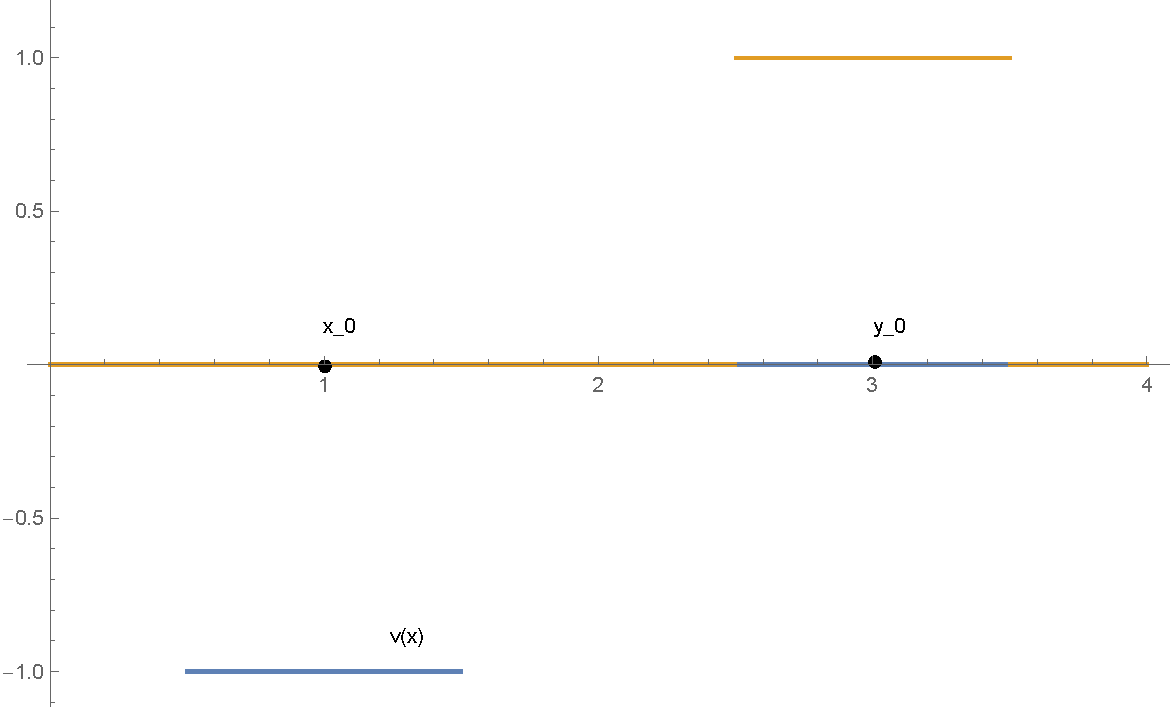
\includegraphics[scale=0.4]{dbr.pdf}
dove v è simmetrica.\\
Allora
\[
	\int_a^b f(x)v(x)\,dx > 0
\]
ASSURDO \qed
\end{dimst}

\begin{dimst}[Per approssimazione]
Si dimostra che ogni funzione $v \in C^0$ a media nulla si può approssimare con funzioni $v \in C^\infty_c((a,b))$ a media nulla e quindi 
\[
	\int_a^b f(x)v(x)\,dx = 0\quad \forall v \in C^\infty_c \text{ con } \int_a^b v(x) = 0 
\]
\[
	\ra \int_a^b f(x)v(x)\,dx = 0 \quad \forall v \in C^0 \text{ con } \int_a^b v(x)\,dx = 0
\]
A questo punto prendo $c \in \bbr $ t.c. $\int_a^b (f(x)+c)\,dx = 0$ e uso $v(x) = f(x)+c$. Ottengo quindi che $f(x) + c \equiv 0 \ra f(x)$ è costante. \qed
\end{dimst}
Anche in questo caso posso usare classi più ristrette di funzioni.\\
\begin{ex}
\[
	min\{\int_0^2 \dot u^2\,dx |\underbrace{ u(0) = 0, u(2) = 5, \int_0^2 u(x)\,dx = 7}_{\bbx}\}
\]
Osserviamo che $\bbx$ è uno spazio affine con giacitura
\[
	V := \{v \in C^1([0,2])|v(0) = 0, v(2) = 0, \int_0^2v(x)\, dx = 0 \}
\]
Data $u \in \bbx$ e $v \in V$ calcolo
\[
	F(u + tv) = F(u) + 2t \int_0^2 \dot u \dot v + t^2\int_0^2\dot v^2
	\ra \delta F(u,v) = \lim_{t\to0} \frac{F(u+tv)-F(u)}t = 2\int_0^2\dot u \dot v
\]
Integrando per parti e supponendo $u \in C^2$ troviamo
\[
	\delta F (u,v) = -2 \int_0^2 \ddot u v
\]
Quindi se u è un punto di minimo deve verificare
\[
	\int_0^2 \ddot u v = 0
\]
\[
	\forall v \in C^1([0,2]) \text{ t.c. } \int_0^2v(x) = 0, v(0)=v(2)=0
\]
Possiamo allora applicare il lemma DBR e quindi $\ddot u = $ costante $\ra u(x) = ax^2+bx+c$.\\
Imponendo le 3 condizioni trovo poi a,b,c.\\
Una volta trovato il punto di minimo faccio la dimostrazione con la disuguaglianza.
\end{ex}
\begin{lem}[DBR altro enunciato]
\[
	\int_a^b f(x)\dot v(x)\, dx = 0\quad \forall v \in C^\infty_c((a,b))
\]
Allora
\[
	f(x) \equiv \text{ c.te in } [a,b]
\]
\end{lem}

\begin{dimst}
Basta osservare che le funzioni $\dot v$ con $v \in C^\infty_c((a,b))$ sono tutte e sole le $w \in C^\infty_c$ a media nulla (l'integrale è ka differenza tra i valori agli estremi).
\end{dimst}

\begin{ex}
\begin{enumerate}
\item{$\int_a^b fv = 0\quad \forall v \in C^\infty_c \text{ t.c. } \int_a^b v = 2017 $}
\item{$\int_a^b f \ddot v = 0\quad v \in C^\infty_c $}
\end{enumerate}
\begin{enumerate}
\item{$f = 0$, la dimostrazione è analoga a quella per v a media nulla}
\item{$f(x)$ è una funzione affine del tipo $ax + b$}
\end{enumerate}
\end{ex}

\begin{oss}
Stiamo con questi lemmi cercando l'ortogonale in $L^2([a,b]) $ di un certo sottoinsieme V.
\end{oss}

\chapter{Lezione 4}
In questo capitolo studiamo la nascita delle condizioni al bordo (BC).\\

\begin{ex}
\[
	F(u)= \int_0^1 \dot{u}^2 + u^2\, dx
\]
\[
	\bbx = \{u \in C^1([0,1]) | u(0) = A, u(1) = B \}	
\]
\[
	F(u + tv) = \int_0^1 (\dot{u} + t \dot{v})^2 + (u + tv) = \int_0^1 (\dot{u}^2 + 2t \dot{u} \dot{v} +t^2 \dot{v}^2 + u^2 +2tuv + t^2v^2)
\]
\[
	\ra \delta F(u, v) = 2 \int (\dot{u} \dot{v} +uv) \qquad{\textbf{1° forma integrale}}
\]
Integrando, poi, per parti otteniamo 
\[
	\delta F(u, v) = 2 \int_{0}^{1}(-\ddot{u}v+uv) = 2 \int_{0}^{1}(-\ddot{u}+u)v \qquad{\textbf{2° forma integrale}}
\]
\begin{oss}
Ricordiamo che i termini di bordo sono nulli poichè $v(0)=v(1)=0$
\end{oss}
\noindent 
Se u è un punto di minimo, allora per FLCV
\[
	-\ddot{u} + u \equiv 0 \ra \underbrace{\ddot{u} = u}_{ELE}, \underbrace{u(0) = A, u(1) = B}_{\text{DBC, Dirichlet Boundary Condition}}	
\]
\end{ex}

\begin{ex}
Consideriamo la stessa $F(u)$, ma adesso $\bbx = \{u \in C^1([0,1])|u(0) = A \} $\\
In questo caso $V = \{v \in C^1([0,1])|v(0) = 0 \} $\\
Allora 
\[
	\delta F(u,v) = 2 \int_{0}^{1} \dot{u} \dot{v} + uv
\]
Integrando per parti allora otteniamo 
\begin{align}
	\delta F(u,v) &=  2 \int_{0}^{1} (-\ddot{u}v + uv) + [\dot{u}	v]_0^1 \\
	& = 2 \int_{0}^{1}(-\ddot{u} +u)v + u(1)v(1)
\end{align}
In questo caso la seconda forma integrale contiene un termine di bordo.\\
Se u è un punto di minimo, allora questa è 0 $\forall v \in V$.\
Procedo in due fasi:\\
1. Mi limito a considerare le v che verificano anche $v(1) = 0$. Ottengo quindi la stessa equazione del primo esempio $\ddot{u}	= u $.\\
2. Adesso l'equazione diventa 
\[
	\dot{u}(1) \dot{v}(1) = 0
\]
allora basta prendere $v \in V$ con $v(1) \not = 0 $ per ottenere che $\dot{u}(1) = 0$\\
Alla fine si ottiene
\[
\begin{cases}
	\ddot{u} = u, & ELE \\
	u(0) = A, & DBC \\
	\dot{u}(1) = 0, & NBC, \text{ Neumann boundary condition}
\end{cases}
\]
Si conclude poi sempre mediante disuguaglianza.
\end{ex}

\begin{ex}
Stessa $F(u)$, $\bbx = \{ u \in C^1([0,1])\}$. Nascono in questo caso le due Neumann agli estremi:
\[
	\begin{cases}
	\ddot{u} = u\\
	\dot{u}(0) = 0\\
	\dot{u}(1) = 0
	\end{cases}
\]
\end{ex}	

\begin{ex}
$\bbx = \{u \in C^1([0,1])| u(0) = u(1)$. In questo caso $\bbx$ è uno spazio vettoriale quindi $V = \bbx$.
\begin{align}
\delta F(u,v) &= 2 \int_{0}^{1}(-\ddot{u}+u)v + 2\dot{u}(1)v(1) - 2\dot{u}(0)v(0)\\
& = 2 \int_{0}^{1}(-\ddot{u}+u)v + 2v(0)(\dot{u}(1) - \dot{u}(0))
\end{align}
Nella prima fase pongo $\ddot{u} = u$, mentre nella seconda prendo v con $v(0)=v(1)\not=0$ ed ottengo $\dot{u}(1)=\dot{u}(0)$.
Devo allora risolvere
\[
	\begin{cases}
	\ddot{u} = u\\
	\dot{u}(0) = \dot{u}(1)\\
	u(0) = u(1)
	\end{cases}
\]
Le ultime due condizioni sono dette \textbf{PBC, Periodic BC}
\end{ex}

\begin{ex}
$\bbx =\{u \in C^1([0,1])| u(0) = u(1) + 5\} \ra V =\{v \in C^1([0,1])| v(0) = v(1)\} $\\
Con lo stesso conto di prima troviamo che $\dot{u}(1) = \dot{u}(0)$ e quindi 
\[
	\begin{cases}
	\ddot{u} = u\\
	\dot{u}(0) = \dot{u}(1)\\
	u(0) = u(1) + 5
	\end{cases}
\]
\end{ex}

\begin{ex}
$\bbx =\{u \in C^1([0,1])| u(\frac12) = A\} \ra V =\{v \in C^1([0,1])| v(\frac12) = 0\} $\\
Quindi
\[
	\frac12 \delta F(u, v) = \int_{0}^{1}(-\ddot{u} + u)v + \dot{u}(1)v(1) - \dot{u}(0)v(0)
\]
Nella prima fase uso v con $v(0)=v(1)=0$ oltre a $v(\frac12)=0$. Allora per FLCV $\ddot{u} = u$.\\
Dalla seconda fase ottengo poi, come NBC, $\dot{u}(1)=\dot{u}(0)=0$.Ottengo quindi
\[
	\begin{cases}
	\ddot{u} = u\\
	\dot{u}(0) = \dot{u}(1) = 0\\
	u(\frac12) = A
	\end{cases}
\]
che sono in generale troppe condizioni.\\
Si verificano quindi due casi:\\
1. C'è la soluzione e con la disuguaglianza posso mostrare che è un minimo;\\
2. Le condizioni sono incompatibili e quindi il minimo non esiste. Ci possiamo quindi chiedere chi sia l'inf.\\
Per rispondere a questa domanda risolvo i problemi separatamente

\[
	\begin{cases}
	\ddot{u} = u\\
	\dot{u}(0) = 0\\
	u(\frac12) = A
	\end{cases}
\]

\[
	\begin{cases}
	\ddot{u} = u\\
	\dot{u}(1) = 0\\
	u(\frac12) = A
	\end{cases}
\]
Accade dunque che in $\frac12$ non si incollano $C^1$.
\end{ex}

\begin{oss}
Se fosse stato $F(u) = \int \ddot{u}^2+ u^2$, allora ELE di ordine 4, cioè il grado di ELE è sempre il doppio dell'ordine di derivazione.
\end{oss}

\begin{oss}
Se nel problema iniziale metto $\dot{u}(0) = 3$ ottengo come sempre che $\ddot{u} = u$ e che 
\[
	\dot{u}(1) v(1) - \dot{u}(0)v(0) = 0 \ra \dot{u}(1) = \dot{u}(0) = 3
\]
quindi non esiste il minimo, ma più in generale se $F(u)$ dipende da u e $\dot{u}$ non posso mettere condizioni su $\dot{u}$.
\end{oss}

\chapter{Lezione 5}
\section{Equazione di Eulero-Lagrange}

Sia
\[
	F(u) = \int_{a}^{b}L(x, \dot{u}, \ddot{u})\, dx
\]
con 
\[
	L : \underbrace{[a,b]}_{\ni x}\times \underbrace{\bbr}_{\ni s}\times\underbrace{\bbr}_{\ni p} \to \bbr
\]
Data $u: [a,b] \to \bbr$ e data $v: [a,b] \to \bbr$ con $v(a)=v(b)=0$ posso definire
\[
	\psi(t) := F(u+tv) = \int_{a}^{b}L(x, u+tv, \dot{u} + t \dot{v})\, dx
\]
e porre 
\[
	\delta F(u,v) := \psi'(0)
\]

\begin{teo}[Integrali dipendenti da parametro]
Sia $[a,b] \subseteq \bbr$ un intervallo, sia $\delta >0$, sia 
\[
	f:[a,b]\times(-\delta, \delta) \to\bbr \qquad x \in [a,b], t\in (-\delta,\delta)
\]
Poniamo 
\[
	\psi(t) := \int_{a}^{b}f(x, t)\,dx
\]
Allora
\begin{enumerate}
\item{Se $f(x,t)$ è continua in $[a,b]\times(-\delta, \delta)$, allora $\psi(t)$ è continua in $(-\delta,\delta)$;}
\item{Se $f_t(x,t)$ è continua in $[a,b]\times(-\delta,\delta)$, allora $\psi$ è derivabile e \\ $\psi '(t) = \int_{a}^{b}f_t(x,t)\,dx$. Cioè la derivata dell'integrale è l'integrale della derivata.}
\end{enumerate}
\end{teo}

Utilizzando il teorema otteniamo che
\[
	\psi '(t) = \int_{a}^{b}L_s(x, u+tv, \dot{u} + t\dot{v})v + L_p(x, u+tv, \dot{u} +t \dot{v}) \dot{v}\, dx
\]
da cui 
\[
	\delta F(u,v) = \psi'(0)=\int_{a}^{b}[L_s(x,u, \dot{u})v + L_p(x, u, \dot{u}) \dot{v}]\,dx
\]
che è quella che avevamo chiamato la \textbf{Prima forma integrale della variazione prima}.\\

\begin{oss}
Abbiamo utilizzato come ipotesi che $L \in C^1$ in s e p, $u \in C^1, v \in C^1$. Non abbiamo ancora utilizzato $v(a)=v(b)=0$, che useremo per la seconda forma.
\end{oss}

Integrando poi per parti il secondo termine troviamo 
\[
	\int_{a}^{b}L_p(x, u, \dot{u}) \dot{v}\,dx = [L_p(x, u, \dot{u})v]_a^b - \int_{a}^{b}[L_p(x, u, \dot{u})]' v\,dx
\]
Se $v(a)=v(b)=0$, il termine di bordo si annulla e troviamo
\[
	\delta F(u,v) = \int_{a}^{b}[L_s(x, u, \dot{u}) - L_p'(x, u, \dot{u})]v\,dx
\]
detta \textbf{Seconda forma integrale della variazione prima}.

\begin{oss}
Qui utilizziamo $L \in C^2, u \in C^2, v \in C^1$ e $v(a)=v(b)=0$.
\end{oss}

Se u è un punto di minimo (tra quelli che hanno lo stesso dato al bordo), allora la $\delta F(u,v) = 0 ~\forall v \in V$. Allora utilizzando il lemma fondamentale ottengo che
\[
	[L_p(x, u, \dot{u})]' = L_s(x, u, \dot{u})
\]
ELE in forma differenziale.

\begin{oss}[Condizione di Neumann in generale]
\[
	u \in argmin\{F(u) | \underbrace{u \in C^1([a,b]), u(a)=A}_{\bbx} \}
\]
Se c'è abbastanza regolarità, usando solo v con $v(a)=v(b)=0$ ritroviamo ELE come sopra.\\
Integrando per parti la prima forma troviamo
\[
	0 = \delta F(u,v) = \int_{a}^{b}\underbrace{[(L_p(x, u, \dot{u}))' - L_s(x, u, \dot{u})]}_{0 \text{ per ELE}}v\,dx + [L_p(x, u, \dot{u})v]_a^b
\]
\[
	\ra L_p(b, u(b), \dot{u}(b))v(b) - L_p(a, u(a), \dot{u}(a))v(a) = 0 
\]
adesso posso mettere $v(a)=0$, ma $v(b)$ può essere $1$, quindi si ha una condizione su $L_p$ in un estremo.
\[
	L_p(x, u, \dot{u}) = 0 \qquad \text{ nell'estremo considerato è detta NBC generale}
\]
\end{oss}

\begin{oss}
L'equazione ELE
\[
	[L_p(x, u, \dot{u})]' = L_s(x, u, \dot{u})
\]
espansa diventa
\[
	L_{px}(x, u, \dot{u}) + L_{ps}(x, u, \dot{u})\dot{u} + L_{pp}(x, u, \dot{u})\ddot{u} = L_s(x, u, \dot{u})
\]
che si può scrivere in forma normale e quindi soddisfa il teorema di Cauchy-Lipschitz se 
\[
	L_{pp}(x, u, \dot{u}) \not = 0 \qquad \forall x \in [a.b]
\]
\end{oss}

\subsection{ELE in forma DBR}
Scrivo la prima forma integrale, introduco la funzione 
\[
	\hat{L}(x) := \int_{a}^{x}L_s(t, u(t), \dot{u}(t))\,dt
\]
e osservo che 
\[
	\int_{a}^{b}L_s(x, u, \dot{u})v = [\hat{L}(x)v(x)]_a^b - \int_{a}^{b} \hat{L}(x)\dot{v}(x)\,dx
\]
Il termine di bordo si annulla e ottengo
\[
	\delta F(u, v) = \int_{a}^{b}[\hat{L}(x) + L_p(x, u, \dot{u})]\dot{v}\,dx
\]
Se u è un punto di minimo/massimo, allora dal lemma DBR otteniamo che
\[
	L_p(x, u, \dot{u}) = c + \int_{a}^{x}L_s(t, u(s), \dot{u}(s))\,ds \quad \text{ ELE-DBR}\footnote{serve meno regolarità in L ed u}
\]

\subsection{ELE in forma ERDMANN}
Consideriamo il caso in cui la Lagrangiana non dipenda da x.
\[
	(L_p(u, \dot{u}))' = L_s(u, \dot{u})
\]
Moltiplico a destra e sinistra per $\dot{u}$ ed ottengo


$$(L_p(u, \dot{u}))'\dot{u} = L_s(u, \dot{u})\dot{u} $$
$$\ra (L_p(u, \dot{u}) \dot{u})' - L_p(u, \dot{u})\ddot{u} = L_s(u, \dot{u}) \dot{u}$$
$$\ra (L_p(u, \dot{u}) \dot{u})' = L_s(u, \dot{u})\dot{u} + L_p(u, \dot{u})\ddot{u}$$
$$\ra (L_p(u, \dot{u}) \dot{u})' = (L(u, \dot{u}))'$$

e quindi
\[
	L_p(u, \dot{u}) \dot{u} = L(u, \dot{u}) + c
\]
questa è detta equazione \textbf{ELE-Erdmann}.

\begin{oss}
Questa è un'equazione differenziale di ordine 1.
\end{oss}
\begin{oss}
ELE classica ed ELE Erdmann \underline{non} sono equivalenti, ma
\[
\text{u soddisfa ELE classica} \ra \text{ u soddisfa ELE-Erdmann}		
\]	
\[
\text{u soddisfa ELE-Erdmann} \ra \text{ u soddisfa ELE classica nei punti } x\in[a,b] \text{ t.c. }  \dot{u}(x) \not= 0 \footnote{Basta fare i passaggi al contrario}
\]
\end{oss}	

\begin{oss}[Piccola generalizzazione]
Consideriamo il caso in cui F dipenda da più derivate successive
\begin{align}
	F(u) & = \int_{a}^{b}L(x, u, \dot{u}, \ddot{u}, \dots, u^{(k)})\,dx \\
	& = \int_{a}^{b}L(x, s, p_1, \dots, p_k)
\end{align}
\[
	\delta F(u, v) = \int_{a}^{b}L_s(\dots)v + L_{p_1}(\dots) \dot{v} + \dots + L_{p_k}(\dots) v^{(k)}
\]
Integrando per parti e supponendo v abbastanza nulla al bordo
\[
 	\delta F(u, v) = \int_{a}^{b}[L_s - (L_{p_1})' + (L_{p_2})''+ \dots]v\,dx
\] 
Quindi se u è un punto di min/max dal FLCV troviamo
\[
	\sum^{k}_{i=1} (-1)^{i+1}\frac{d^i}{dx^i}L_{p_i}(x, u, \dot{u}, \dots, u^{k}) = L_s(x, u, \dot{u}, u^{k})
\]
che è la ELE per dipendenza da più derivate.
\end{oss}

\chapter{Lezione 6}
\section{Come dimostrare che u è un minimo di F}
Alcune strategie possibili:\\
\begin{enumerate}
\item Convessità
\item Lemma trivial
\item Calibrazioni
\item Campi di Weierstrass
\end{enumerate}

\subsection{Convessità}
Da analisi 1 sappiamo che: se $f:[c,d]\to\bbr$ è una funzione convessa e $x_0 \in (c,d)$, allora esiste una costante $m\in\bbr$ tale che 
\[
	f(x)\ge f(x_0)+m(x-x_0)\quad\forall x \in [c,d]
\]
In generale basta prendere $m \in [f_-'(x_0), f_+'(x_0)]$.\\
Da analisi 2 sappiamo che: se $f(x,y)$ è convessa e se $(x_0, y_0)\in \bbr$, allora esistono $m_1\in\bbr, m_2\in\bbr$ t.c.
\[
	f(x, y)\ge f(x_0, y_0) + m_1(x-x_0) + m_2(y-y_0)\quad \forall(x,y)\in\text{Dominio}
\]

\begin{teo}
Consideriamo adesso $F(u) = \int_{a}^{b}L(x, u, \dot{u})\,dx$ con DBC.\\
Supponiamo che:\\
\begin{enumerate}
\item Ci sia abbastanza regolarità
\item $u_0(x)$ sia soluzione di ELE con DBC
\item $\forall x \in [a,b]$ la funzione $(s,p)\to L(x, s, p)$ è convessa come funzione di due variabili.
\end{enumerate}
Allora $u_0$ è un punto di minimo per il problema con le DBC.
\end{teo}

\begin{dimst}
Prendo un qualunque altro competitore w e pongo $v(x) := w(x)-u(x)$ ed osservo che $v(a)=v(b)=0$. Scrivo che 
\[
	F(w) = F(u_0 + v) = \int_{a}^{b} L(x, u_0 + v, \dot{u_0} + \dot{v})\,dx
\]
Dopodichè dalla convessità e regolarità di L ottengo la disuguaglianza
\[
	L(x, s +s_1, p+p_1)\ge L(x, s, p) + L_s(x, s, p)s_1 + L_p(x, s, p)p_1
\]
Prendendo poi $s = u_0 , s_1 = v, p = \dot{u}_0, p_1 = \dot{v}$ si ha che
\[
	F(w)\ge \int_{a}^{b}L(x, u_0, \dot{u}_0) + \underbrace{L_s(x, u, \dot{u}_0)v + L_p(x, u_0, \dot{u}_0)\dot{v}}_{= 0 \text{ per la prima forma integrale di ELE}}
\]
\[
	\ra F(w)\ge \int_{a}^{b}L(x, u_0, \dot{u_0}) = F(u_0) \qed
\]
\end{dimst}

\begin{oss}
Abbiamo in realtà usato solo che $u_0$ risolve la prima forma integrale di ELE, che richiede meno regolarità su L. Inoltre, se L fosse strettamente convessa in $(s, p)$, allora la disuguaglianza di analisi 2 è stretta se $(x, y) \not = (x_0, y_0)$, da cui l'unico modo per avere uguaglianza è che v e $\dot{v}$ siano nulle, cioè $v(x) \equiv 0$. Quindi $u_0$ è l'unico punto di minimo. 
\end{oss}

\begin{ex}
$$
F(u) = \int_{0}^{1} (\dot{u}(x))^4\, dx
$$
e minimizzo con $u(0) = 0, u(1) = 5$. Allora
\[
	L(x, s, p) = p^4 \ra [L_p(x, s, p)]' = L_s(x, s, p) \ra (4 \dot{u}^3)' = 0 \ra \dot{u} = c.te\ra u = \text{retta}
\]
Per l'enunciato precedente, la retta è l'unico punto di minimo; tuttavia se non pensiamo alla convessità è meno evidente:
\[
	F(w) = F(u+v) = \int_{0}^{1}(\dot{u} + \dot{v})^4 = \int_{0}^{1}(\underbrace{\dot{u}^4}_{=F(u)} + \overbrace{4\dot{u}^3 \dot{v}}^{=0 \text{ integrando per parti ed usando ELE}} + \underbrace{6 \dot{u}^2 \dot{v}^2 + 4 \dot{u} \dot{v}^3 + \dot{v}^4}_{\ge \text{ ma non del tutto evidente}\footnote{Forma quadratica definita positiva, tutttavia fare i conti non è sempre una buona idea. Questa volta ci salva l'esponente basso}})
\]
\end{ex}

\begin{lem}[Lemma trivial]
Sia $\bbx$ un insieme, e siano $F:\bbx \to\bbr$ e $G:\bbx\to\bbr$ due funzioni. Supponiamo che
\begin{enumerate}
\item $F(x) \ge G(x) \quad \forall x\in \bbx$
\item $x_0 \in \bbx$ è punto di minimo di G
\item $F(x_0) = G(x_0)$ 
\end{enumerate}
Allora $x_0$ è punto di minimo per F.
\end{lem}

\begin{dimst}
\[
	\forall x \in \bbx \text{ vale: } F(x)\underbrace{\ge}_{1}G(x)\underbrace{\ge}_{2} G(x_0)\underbrace{=}_{3}F(x_0)\qed
\]
\end{dimst}

\begin{ex}
Consideriamo il funzionale $F(u) = \int_{o}^{2}(\dot{u}^2 - 1)^2\,dx$ e l'insieme $\bbx = \{ u \in C^1([0,2])| u(0)=1, u(2)=7\}$. In questo caso la Lagrangiana non è convessa in p come si evince dalla figura$\qquad$
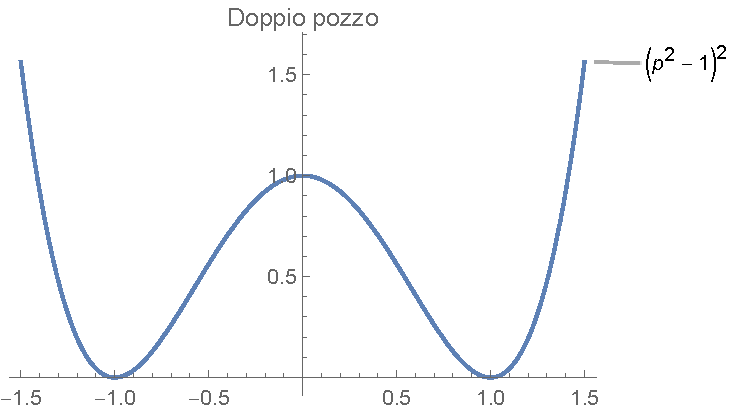
\includegraphics[scale=0.4]{doppio-pozzo.pdf}.\\
Supponiamo adesso che la retta $u_0(x) := 1 +3x$ sia l'unico punto di minimo e troviamo la G giusta.\\
\textit{Idea:} convessifico L. Considero
\[
	\hat{L}(p) = \begin{cases}
	L(p) & |p|\ge 1 \\
	0 & |p| \le 1
	\end{cases}
\]
ed osservo che $\hat{L}$ è convessa. Pongo
\[
	G(u) := \int_{0}^{2} \hat{L}(\dot{u})\,dx
\]
e verifico le ipotesi.\\
(1) segue da $L \ge \hat{L}$; (2) segue dalla convessità di $\hat{L}$, quindi $u_0$ è punto di minimo per G; (3) segue dal fatto che $L(3) = \hat{L}(3)$. Da questo segue che $u_0$ è punto di minimo per F. Inoltre G ha come unico minimo $u_0$, in quanto $\hat{L}$ strettamente convessa in un intorno di $p=3$, quindi $u_0$ è l'unico punto di minimo di G.
\end{ex}

\begin{oss}
Cosa succede nell'esempio se $\bbx = \{ u \in C^1([0,1])| u(0)=1, u(1)=2\}$?\\
In questo caso la retta $u_0(x) = 1 + \frac12 x$ non è punto di minimo, anzi il minimo non esiste e l'inf è 0.\\
\begin{figure}[h]
\centering
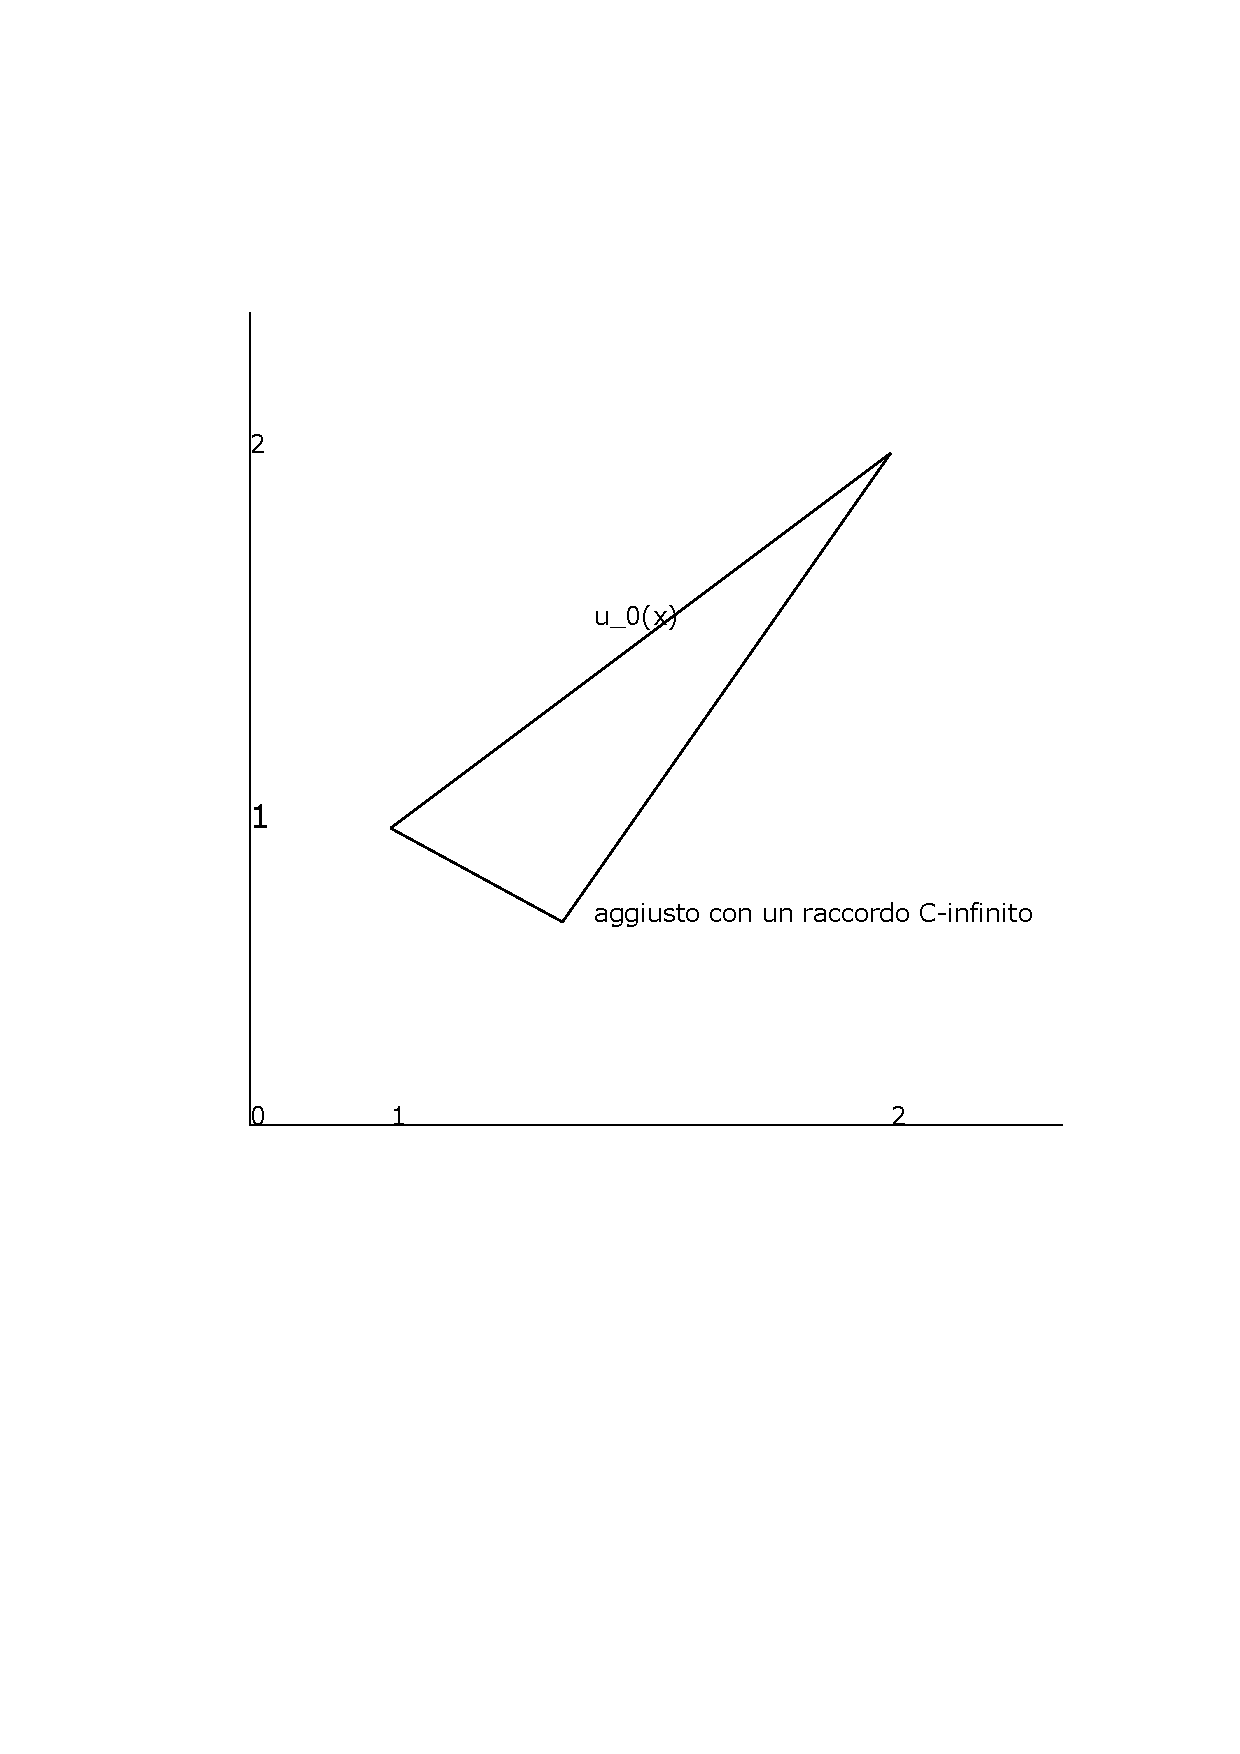
\includegraphics[scale=0.3]{capitolo6.pdf}
\end{figure}
\end{oss}

Minimizziamo adesso $F(u) = \int_{0}^{2}[(\dot{u}^2-1)^2 + \underbrace{(u-1-\frac12 x)^2}_{\text{in questo caso pago se mi allontano da $u_0(x)$}}]$. L'inf resta 0.

\chapter{Lezione 7}
\section{Transversality and Point-to-Curve problems}

\begin{defn}[Point to curve problem]
\begin{table}[h]
\begin{minipage}[]{0.49\linewidth}
\begin{flushleft}
Sia dato un punto $(a, A)\in \bbr^2$ e sia data una funzione $\varphi :\bbr\to\bbr$. Consideriamo
\[
	F(u) = \int_{a}^{b}L(x, u, \dot{u})\,dx
\]	
\end{flushleft}
\end{minipage}
\hspace{10mm}
\begin{minipage}[]{0.49\linewidth}
\begin{flushright}
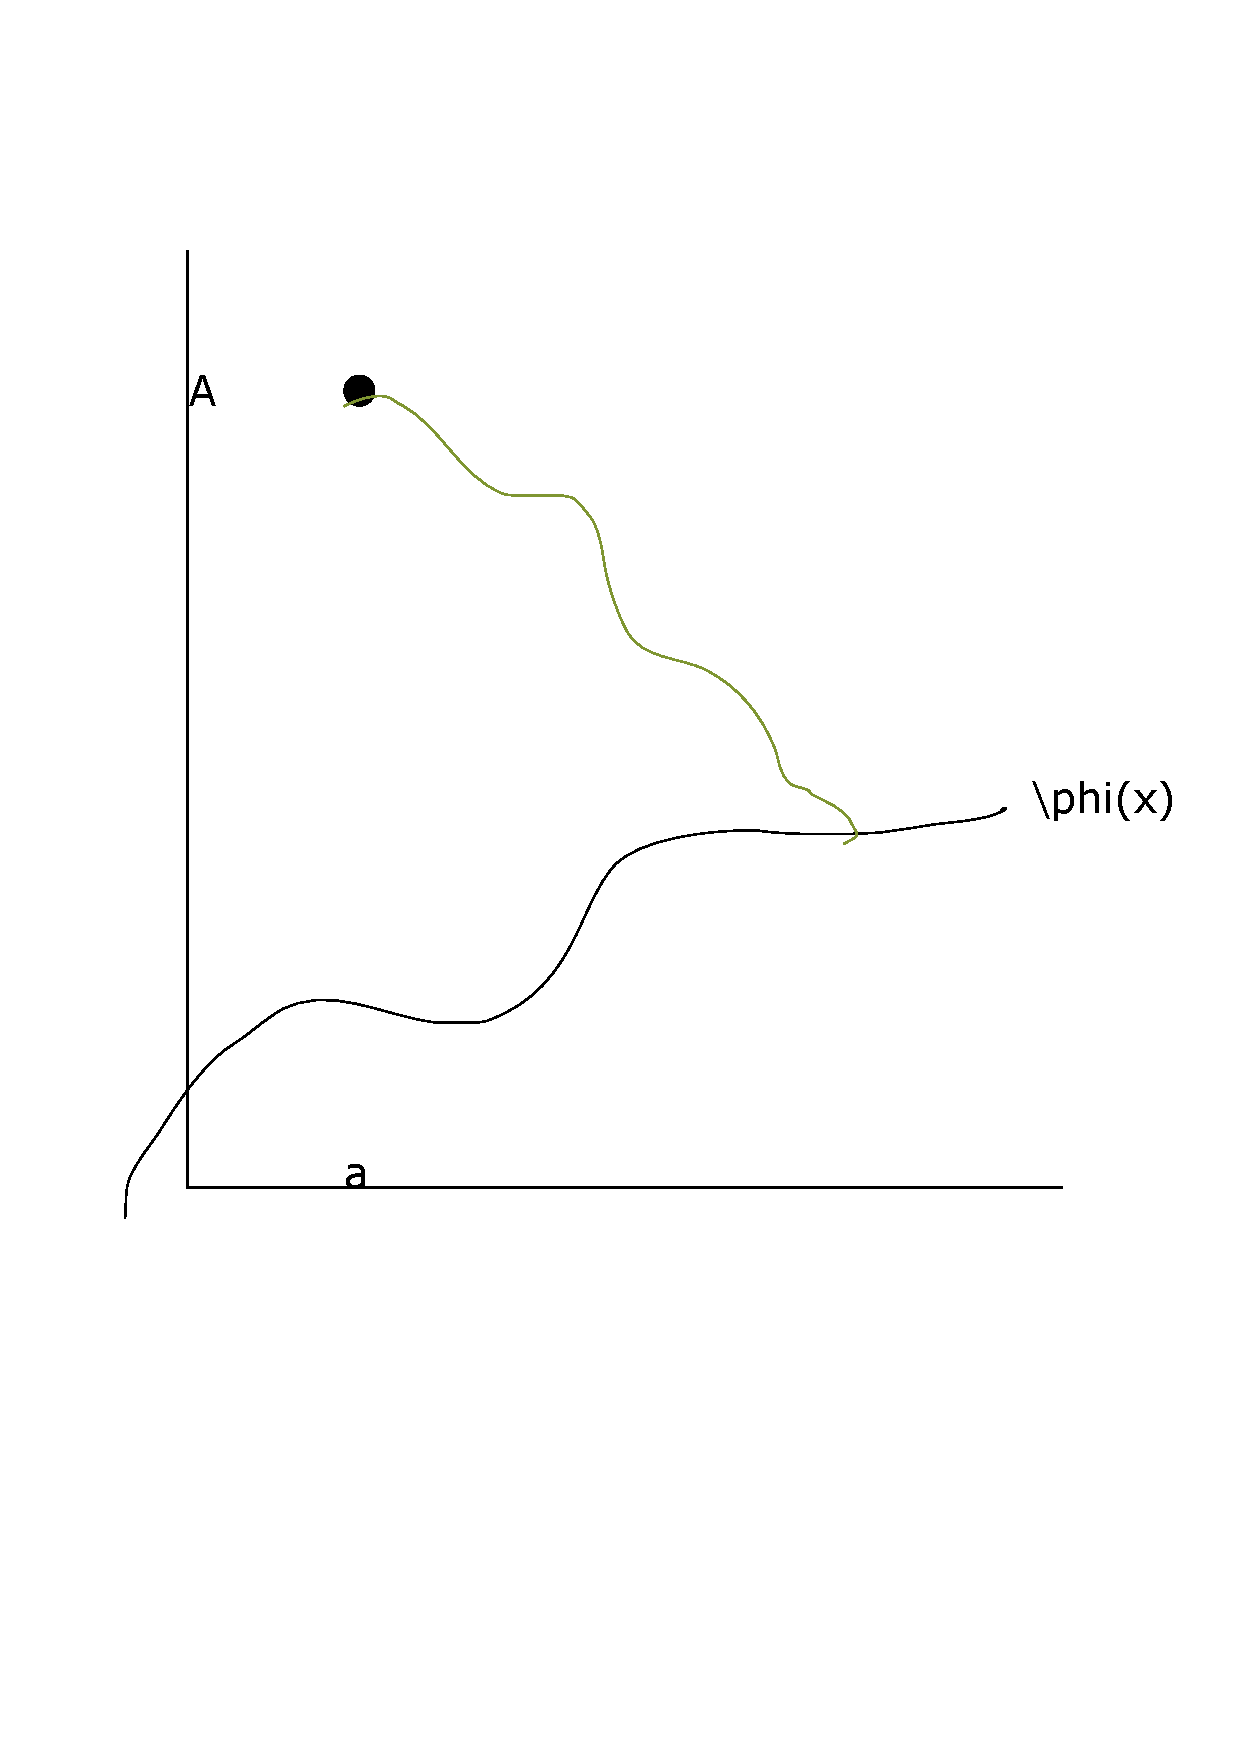
\includegraphics[scale=0.2]{capitolo7.pdf}
\end{flushright}
\end{minipage}
\end{table}

Voglio minimizzare F(u) tra tutte le coppie (u, b) tali che
\[
	u \in C^1([a,b]), u(a)=A, u(b) = \varphi(b)
\]
l'ultima condizione implica che il punto terminale sia sul grafico di $\phi(x)$.
\end{defn}

\begin{oss}
Può essere che b non sia la prima intersezione.
\end{oss}

Vogliamo trovare l'equazione di Eulero-Lagrange in questo caso.

\begin{teo}[Transversality condition]
Se $L \in C^2, \varphi \in C^2$ e $(u_0, x_0) $ minimizza, allora
\[
	[L_p(x, u_0, \dot{u}_0)]'=L_s(x, u_0, \dot{u}_0)\qquad\forall x \in (a, x_0)\text{ : solita ELE}
\]
\[
	u_0(a) = A \text{ : solita DBC}
\]
\[
	L_p(x, u_0(x_0), \dot{u}_0(x_0))[\dot{u}_0(x_0) - \dot{\varphi}(x_0)] = L(x_0, u_0(x_0), \dot{u}_0(x_0))]
\]
L'ultima condizione è detta \textbf{transversality}.
\end{teo}

\begin{oss}
Se $\varphi$ fosse una retta verticale (ma non lo può essere poichè deve essere funzione di x), verrebbe $\dot{\varphi}(x_0) = \infty$ da cui la classica NBC $L_p(x, u_0(x_0), \dot{u}_0(x_0))=0$
\end{oss}

\begin{dimst}
Consideriamo una funzione u(x) ed un punto $x_0$. Consideriamo poi $u + tv$ per una opportuna v(x) che intersecherà $\varphi(x)$. Sia x(t) il punto d'intersezione tra v e $\varphi$.\\
Esistenza ed unicità di x(t) è una questione di teorema delle funzioni implicite, cioè considero 
\[
	\Phi(x, t) := u(x) + tv(x) - \varphi(x)
\]
ed osservo che $\varphi(x_0, 0) = 0$ e spero che per $t \in (-\delta,\delta)$ io possa ricavare x in funzione di t.
\[
	\Phi_t(x, t) = v(x)\quad \Phi_x(x, t) = \dot{u}(x) + t \dot{v}(x) - \dot{\varphi}(x)\ra\Phi_x(x_0, 0) = \dot{u}(x_0) + \dot{\varphi}(x_0)
\]
Se $\dot{u}(x_0) - \dot{\varphi}(x_0) \not = 0$, allora posso ricavare. A questo punto pongo
\[
	\psi(t) := \int_{a}^{x(t)}L(x, u+tv, \dot{u}+t \dot{v})\, dx\ra \psi'(0)=0\footnote{Punto di minimo}.
\]
Quindi
\[
	\psi'(t) = \int_{a}^{x(t)} L_t + L(x(t), u(x(t))+tv(x(t)), \dots) \dot{x}(t)
\]
\[
	\ra \psi'(0) = \int_{a}^{x_0} [L_s(x, u, \dot{u})v + L_p(x, u, \dot{u}) \dot{v}]\, dx + L(x_0, u(x_0), \dots) \dot{x}(0) 
\]
\[
	= \int_{a}^{x_0} [L_s - L_p']v + [L_p(x, u, \dot{u}) \dot{v}]_a^{x_0} + L(x_0, u(x_0), \dots) \dot{x}(0) 
\]
Dal teorema delle funzioni implicite ricavo che 
\[
	\dot{x}(t) = - \frac{\Phi_t(x(t), t)}{\Phi_x(x(t), t)} \leadsto	\dot{x}(0) = -\frac{v(x_0)}{\dot{u}(x_0) - \varphi(x_0)}
\]	
Sostituendo
\[
	\psi'(0) = \int_{a}^{x_0}[L_s - L_p']v + L_p(x_0, u(x_0), \dot{u}(x_0)) \dot{v}(x_0) + L(x_0, u(x_0), \dot{u}(x_0))(-\frac{v(x_0)}{\dot{u}(x_0) - \varphi(x_0)})
\]
Adesso utilizzo funzioni v t.c. $v(x_0)=0$ e da FLCV deduco ELE in (a, $x_0$).\\
Scelgo poi v con $v(x_0)=1$ e ottengo
\[
	L_p(x_0, u(x_0), \dot{u}(x_0)) = \frac{L(x_0, u(x_0), \dot{u}(x_0))}{\dot{u}(x_0) - \dot{\varphi}(x_0) }
\]
Moltiplicando ho la transversality.\\
Passo 2: Supponiamo $\dot{u}(x_0) = \dot{\varphi}(x_0) $.\\
Geometricamente questo significa che l'attacco è "smooth". Uso allora, come competitore, anzichè $u+tv$, la u "allungata".
\[
 	\psi(t) := \int_{a}^{x_0}L(x, u, \dot{u}) + \int_{x_0}^{x_0 + t}L(x, \varphi, \dot{\varphi}) 
 \] 
 \[
 	\psi'(t) = L(x_0 + t, \varphi(x_0 + t), \dot{\vp}(x_0 + t))
 \]
\[
	\ra \psi'(0) = L(x_0, \varphi(x_0), \dot{\vp}(x_0)) = L(x_0, u(x_0), \dot{u}(x_0))
\]

\begin{oss}
Non posso dire che $\psi'(0)=0$ poichè $\psi$ è definita solo per $t \ge 0$.
\end{oss}
Posso dire solo che $\psi'(0)\ge0$ da cui $L(x_0, u(x_0), \dot{u}(x_0))\ge0$.\\
Passo 3: cerco di "accorciare" la u.\\
\textit{inserire immagine minuto 31}\\
In questo caso $\psi(t) = $ funzionale calcolato sulla u accorciata:
\[
	\psi(t) \int_{a}^{x_0 - 2t}L(x, u, \dot{u}) + \int_{x_0-2t}^{x_0-t}L(x, l, \dot{l})
\]
con l: equazione della retta di raccordo
\[
	\ra \psi(t) = \int_{a}^{x_0}L(x, u, \dot{u}) - \int_{x_0-2t}^{x_0}L(x, u, \dot{u}) +  \int_{x_0-2t}^{x_0-t}L(x, l, \dot{l})
\]
Il primo termine è costante, quindi quando derivo sparisce.\\
La derivata del secondo termine è 
\[
	-2L(x_0 - 2t, u(x_0-2t), \dot{u}(x_0-2t))
\]
Perciò quando metto t = 0 ottengo $-2 L(x_0, u(x_0), \dot{u}(x_0)$.\\
Per derivare l'ultimo termine posso scrivere l'equazione di l come retta passante per due punti, oppure osservo che per il teorema della media integrale vale 
\[
	\int_{x_0- 2t}^{x_0-t}L(x, l(x), \dot{l}(x)) = t L(x(t), l(x(t)), \dot{l}(x(t)))
\]
Dividendo per t e passando al limite per $t \to 0$, la derivata del terzo termine è
\[
	L(x_0, u(x_0), \dot{u}(x_0))
\]
poichè $x_0 -2t\le x(t)\le x_0-t$ e $l(x(t)) \in [u(x_0-2t, u(x_0-t))] $. Per passare al limite $\dot{l}(x(t)) \to \dot{u}(x_0)$ serve che $\dot{u}(x_0) = \dot{\varphi}(x_0)$.\\
In conclusione
\[
	\psi'(t) = -L(x_0, u(x_0), \dot{u}(x_0)) \ge 0\quad\text{per }t\ge0
\]
Questo completa la dimostrazione anche nel caso in cui $\dot{u}(x_0) = \dot{\varphi}(x_0)$. \qed
\end{dimst}

\begin{ex}
\[
	F(u, b) = \int_{0}^{b}(\dot{u}^2 + u^2)\, dx
\]
e prendiamo come DBC $u(0) = 1, \varphi(x)\equiv 0 $.\\

\begin{tikzpicture}[scale=1.2]
\draw[->] (-1, 0)  -- (2.5, 0);
\draw[->] (0, -1)  -- (0, 1.5);
\draw (0, 1) node[anchor = north east] {1} .. controls (1/4, 1/6) and (3/2, 1/8) .. (2, 0) node[anchor = south west]{b};
\end{tikzpicture}
Esiste il minimo?\\
ELE: $$L_p' = L_s \ra (2\dot{u})' = 2u \ra \ddot{u} = u \ra u(x) = a cosh(x) + b sinh(x)$$
Da $u(0) = 1$ ottengo che 
\[
	u(x) = cosh(x) + bsinh(x)
\]
Impongo adesso la transversality
\[
	L_p(x, u, \dot{u}) (\dot{u} - \dot{\varphi} ) = L(x, u, \dot{u})\quad\text{in }x_0	
\]
\[
	\ra 2\dot{u}(\dot{u} - 0) = \dot{u}^2 + u^2 \ra \dot{u}^2 = u^2
\]
Nel punto di contatto vale $u(x_0) = 0$, quindi $\dot{u}(x_0)=0$.
\[
 	\ra 
 	\begin{cases}
 	u(x_0) = 0 \\
 	\dot{u}(x_0) = 0
 	\end{cases}
 \] 
 Questo sistema non ha soluzione, in quanto implicherebbe
 \[
 	b = - \frac{sinh(x_0)}{cosh(x_0)} = -\frac{cosh(x_0)}{sinh(x_0)} \ra sinh^2(x_0) = cosh^2(x_0)\to \text{impossibile}
 \]
\end{ex}

\chapter{Lezione 8}
\section{Road map metodo indiretto}
\begin{enumerate}
	\item Determino condizioni necessarie: ELE + BC
	\item Spero di essere capace di risolverle
	\item Spero di riuscire a dimostrare che le soluzioni sono minimi via convessità o via funzionale ausiliario
\end{enumerate}

\section{In quale classe ambientare i problemi?}
$$ F(u) = \int_{a}^{b} L(x, \dot{u}, \ddot{u})$$
Sia L continua in (x,s,p). Supponiamo di avere DBC (ma cambia poco se non ci sono). I possibili ambienti per il problema sono:
\begin{enumerate}
	\item $ u \in C^1 $
	\item $ u \in C^\infty $
	\item $ u \in C^1 $ a tratti
\end{enumerate} 

\begin{teo}
	L'inf di F(u) nelle tre classi è lo stesso.
\end{teo}

\begin{dimst}
	E' facile conseguenza di un lemma di approssimazione.\\
	Ogni funzione $ C^1 $ a tratti si può approssimare con una successione $ {u_n} $ di funzioni $ C^\infty $, dove si intende che 
	\[
	u_n \to u \text{ unif in } [a,b]\]
	\[
	\dot{u}_n \to \dot{u} \text{ unif sui compatti contentìuti in } [a,b] \setminus \{ \text{ punti di discontinuità della derivata prima } \} \]
	\[
	\exists M \in \bbr \: t.c.\: |\dot{u}_n(x)|\le M \; \forall x \in [a,b] \forall n \in \mathbb{N}
	 \]
\end{dimst}

\begin{ex}
	Data $ f:[a.b] \to\bbr$, risolvere
	\[ min\{\int_{a}^{b} \dot{u}^2 + (u-f)^2 | u \in C^1([a,b])\} \]
	ELE: $ (L_p)' = L_s \leadsto  \ddot{u} = u-f$ che per molte classi di f si sa risolvere esplicitamente.\\
	In ogni caso, per ogni f continua, esiste una famiglia a due parametri di soluzioni:\\
	\[ u(x)  = a\cosh (x) +b \sinh (x) +  \bar{u}(x) \]
	con $ \bar{u}(x) $ soluzione qualunque dell'eq. non omogenea.
	Nascono così le NBC: $L_p = 0$ al bordo, quindi $\dot{u}(a) = \dot{u}(b) = 0$.
	\\
	Questo sistema ha quindi un'unica soluzione ed essa è un punto di minimo perchè $L(x,s,p) = p^2 + (s-f(x))^2$ è strettamente convessa nella coppia (s,p) e quindi la matrice Hessiana è definita positiva.
	

\end{ex}

\begin{prop}[Proprietà qualitativa della soluzione]
	$$max\{u(x)|x \in [a,b]\} \le max\{f(x)|x \in [a,b]\}$$
	$$min\{u(x)|x \in [a,b]\} \ge min\{f(x)|x \in [a,b]\}$$
	
	
\end{prop}

\begin{proof}[Variazionale]
	Usiamo il solito argomento di troncamento: al minimo $u_0(x)$ non conviene andare sopra $f(x)$ perchè se tronco "risparmio" su $\dot{u}^2$ e su $(u-f)^2$. In altre parole, supponiamo esista $x_0 \in (a,b)$ t.c. $u(x_0)> max(f(x))$.\\
	Siano $x_1 < x_0 < x_2$ t.c. $u(x_1) = max(f(x))$ e $u(x_2) = max(f(x))$, allora
	$$
	\bar{u}(x)=
	\begin{cases}
		u(x) & \text{ fuori da } [x_1, x_2]\\
		max(f) & \text{ in } [x_1,x_2]
	\end{cases}
	$$
	Allora $F(\bar{u})<F(u)$ con $\bar{u}$ ammissibile poichè $C^1$ a tratti.\\
	Se $x_1, x_2$ in qualche modo non esistono posso prendere $x_1 = a, x_2 = b$
\end{proof}

\begin{oss}
	Prendere $\bar{u}(x) := min\{u(x), maxf\}$ è pericoloso perchè non è detto che sia $C^1$ a tratti.
\end{oss}

\begin{ex}
	$$min\{\int_{-1}^{1}\dot{u}^4 + u | u(-1)=u(1)=0\} $$
	ELE: $(L_p)' = L_s \ra (4\dot{u}^3)' = 1 \ra 12 \dot{u}^2\ddot{u} = 1$\\
	Si risolve ponendo $\dot{u}=v$.\\
	Oppure osserviamo che la Lagrangiana è autonoma $\leadsto$ ELE in forma Erdmann.
	$$ L_p(x, u, \dot{u})\dot{u} = c + L(x,u,\dot{u})$$
	$$ 4 \dot{u}^3\dot{u} = c + \dot{u}^4 + u$$
	$$\dot{u} = \pm\sqrt[4]{\frac u3 + c}$$
	Per concludere osserviamo che u risolve ELE anche in una forma molto debole (prima forma integrale) e che $L(x,s,p) = p^4 - s$ è convessa nella coppia (s,p) anche se non strettamente.
\end{ex}

\begin{oss}
	Il minimo in questione è $C^1$ ma non $C^2$; risolve ELE nella forma $(4\dot{u}^3)' = 1$, ma non nella forma $12 \dot{u}^2 \ddot{u} = 1$. Questo è dovuto al fatto che $L_{pp}$ si annulla.
\end{oss}


\chapter{Lezione 9}
\section{Metodo diretto}
Vogliamo dimostrare l'esistenza del minimo (ci muoveremo su spazi di Hilbert, metrici o dotati di nozione di convergenza), non necessariamente trovarlo.

\begin{defn}[Nozione di convergenza]
	Dato un insieme $\bbx$, una nozione di convergenza è \textit{dichiarare le successioni convergenti ed i relativi limiti}. Più formalmente, detto
	$$
	S_{eq}(\bbx) = \{\text{successioni in }\bbx\} = \{f:\mathbb{N} \to \bbx \}
	$$
	Una nozione di convergenza è un sottoinsieme qualunque di $S_{eq}\times\bbx$
\end{defn}

\begin{oss}
	Il sottoinsieme può essere di qualunque tipo:
	\begin{itemize}
		\item Successioni costanti che tendono ad altro
		\item Successioni che hanno infiniti limiti
		\item Successioni convergenti con sottosuccessioni che tendono ad altro
	\end{itemize}
\end{oss}

\begin{defn}[Insieme compatto]
	Un sottoinsieme $K\subset\bbx$ di dice compatto (per successioni) se ogni successioni a valori in K ammette almeno una sottosuccessione che converge ad un elemento di K.
\end{defn}

\begin{defn}
	Una funzione $f:\bbx\to\bbr$ si dice
	\begin{itemize}
		\item \underline{Continua} se per ogni successione $x_n\to x_\infty$ in $\bbx$ vale $f(x_n)\to f(x_\infty)$
		\item \underline{Semicontinua inferiormente} se per ogni successione $x_n \to x_\infty$ in $\bbx$ vale $$\liminf_{n\to\infty} f(x_n)\ge f(x_\infty)$$. Analogamente si definiscono le semicontinue superiormente.
	\end{itemize}
\end{defn}

\begin{teo}[Weierstrass]
	Sia $f:\bbx\to\bbr$. Supponiamo $\bbx$ compatto ed f SCI rispetto alla stessa nozione di convergenza. Allora f ammette minimo.
\end{teo}

\begin{proof}
	Poniamo $I := inf\{f(x)|x\in \bbx\}$ che esiste necessariamente in $\bbr \cap \{-\infty\}$. Per un lemma di analisi 1 $\exists\{y_n\}\subseteq f(\bbx)$ t.c. $y_n \to I$. Per definizione di immagine $\exists \{x_n\}\subseteq \bbx$ t.c. $y_n = f(x_n)$. Poichè $\bbx$ è compatto $\exists x_{n_k} \to x_\infty$. Allora $$I\le f(x_\infty)\le \liminf_{k\to\infty} f(x_{n_k}) = \liminf_{k\to\infty} y_{n_k} = lim_{n\to\infty} y_n = I$$ perchè $y_n$ ha limite. Allora $f(x_\infty) = I \in \bbr$ \qedhere
\end{proof}

\begin{oss}
	Le due richieste del teorema sono antitetiche.
	\begin{itemize}
		\item Se ho tante successioni convergenti, allora è facile trovare $\bbx$ compatto, ma difficile trovare f SCI
		\item Se ho poche successioni convergenti, è facile trovare f SCI, ma difficile trovare $\bbx$ compatto.
	\end{itemize}
\end{oss}

\begin{defn}[Funzione coerciva]
	Una $f:\bbx\to\bbr$ si dice coerciva se $\exists K\subseteq \bbx$ compatto t.c. $inf\{f(x)|x\in K\} = inf\{f(x)| x \in \bbx\}$
\end{defn}

\begin{coroll}
	Se $f:\bbx\to\bbr$ è coerciva e SCI, allora esiste il minimo.
\end{coroll}

\begin{dimst}
	$$\inf_{x\in\bbx} f(x) =^1 \inf_{x\in K} f(x) =^2 \min_{x \in K} f(x)$$
	1. Per coercitività\\
	2. Per Weierstrass \qedhere
\end{dimst}

\begin{coroll}
	Se $f: \bbx\to\bbr$ è SCI ed esiste un sottolivello contenuto in un compatto e non vuoto, cioè
	$$
	\exists M \in \bbr \: \exists K \subseteq \bbx \text{ compatto } : \varnothing \not= \{x \in \bbx | f(x) \le M\} \subseteq K
	$$
	Allora esiste il minimo
\end{coroll}

\begin{proof}
	Uso il corollario precedente con questo K \qedhere
\end{proof}

\begin{coroll}
	Sia $f: \bbr^n \to \bbr$ SCI e tale che $$\lim_{|x|\to +\infty}f(x) = +\infty$$ Allora esiste il minimo
\end{coroll}

\begin{dimst}
	Tutti i sottolivelli sono chiusi e limitati e quindi contenuti in un compatto.
\end{dimst}

\section{Spazi di Hilbert}
\begin{defn}[Spazio di Hilbert]
	Uno spazio di Hilbert H è uno spazio vettoriale munito di prodotto scalare definito positivo $< \dot , \dot >$ da cui deriva una norma $|x| = \sqrt{<x,x>}$ da cui deriva infine una distanza ($d(x,y) = |x-y|$)rispetto allora quale H diventa uno spazio metrico completo.
\end{defn}

\begin{oss}
	Dalla metrica segue una nozione di convergenza: $$ x_n \to x_\infty \iff |x_n - x_\infty| \to 0$$
\end{oss}

\begin{defn}[Spazio separabile]
	Uno spazio di Hilbert si dice separabile se esiste $D\subseteq H$ denso e numerabile.
\end{defn}

\begin{defn}[Base ortonormale]
	Un sottoinsieme $\{e_n\} \subseteq H$ si dice base hilbertiana o base ortonormale se 
	$$<e_i, e_j> = \delta_{ij}$$
	$$Span\{e_n\} \text{ è denso in } H$$
\end{defn}


\begin{teo}
	Se H è un Hilbert separabile allora ammette almeno una (ma in realtà infinite) base ortonormale
\end{teo}

\begin{defn}[Componente di un vettore]
	Dato un vettore $v \in H$ ed una base ortonormale $\{e_n\}$ allora $$v_k := <v, e_k>$$ si dice componente di v rispetto ad $e_k$
\end{defn}

\begin{prop}
	Sia H un Hilbert con base ortonormale $\{e_n\}$. Allora le componenti hanno le seguenti proprietà 
	\begin{itemize}
		\item $$|v|^2 = \sum_{n = 1}^{\infty}v_n^2 = \sum_{n=1}^{\infty} <v,e_n>^2$$
		\item $$<v,w> = \sum_{n=1}^{\infty}v_n w_n$$
	\end{itemize}
\end{prop}

\begin{teo}
	Se H ammette una base ortonormale allora c'è una corrispondenza biunivoca tra i $v \in H$ e le successioni $\{v_n\}$ di numeri reali a quadrato sommabile, posso cioè identificare ogni vettore con le sue componenti (oppure, posso vedere ogni Hilbert separabile come $\bbr^\infty$).  
\end{teo}

\begin{prop}
	Sia $\{e_n\}$ una base ortonormale in H e sia $\{v_n\}$ una successione di numeri reali. Allora 
	$$ \sum_{n=1}^{\infty}v_n e_n \text{ converge in H }\iff \sum_{n=1}^{\infty} v_n^2$$
\end{prop}

\begin{dimst}
	Sia 
	$$S_n = v_1e_1 + \dots + v_ne_n \textit{ vettore}$$
	$$\hat{S}_n = v_1^2 + \dots + v_n^2 \textit{ numero}$$
	Dati due interi m>n vale 
	$$|S_m - S_n|^2 = |v_{n+1}e_{n+1} + \dots + v_m e_m |^2 = \text{ per ortonormalità } = v_{n+1}^2 + \dots + v_m^2 = \hat{S}_m - \hat{S}_n$$
	Di conseguenza 
	$$\sum_{n=1}^{\infty}v_ne_n \text{ converge in H } \iff \{S_n\} \text{ è di Cauchy in H }$$ $$\iff \{\hat{S}_n\} \text{ è di Cauchy in }\bbr\iff \sum_{n=1}^{\infty}v_n^2 \text{ converge in }\bbr$$
\end{dimst}

\chapter{Lezione 10}
\section{Convergenza forte e debole negli spazi di Hilbert}
\begin{defn}[Convergenza forte]
	Sia H uno spazio di Hilbert, diciamo che $$x_n \to x_\infty$$ se $$|x_n - x_\infty|| \to 0$$
\end{defn}

\begin{prop}
	La norma è continua rispetto alla convergenza forte, cioè $$x_n \to x_\infty \ra ||x_n||\to ||x_\infty||$$
\end{prop}

\begin{proof}
	$$ \big| \, ||x_n|| - ||x_\infty|| \, \big| \le ||x_n - x_\infty||$$ per disuguaglianza triangolare.
\end{proof}

\begin{oss}
	Se H ha dimensione infinita allora le palle chiuse non sono compatte.
\end{oss}

\begin{proof}
	Suppniamo esista una base ortonormale $\{e_n\}$ infinita, osserviamo che $\{e_n\}$ è una successione di vettori contenuti nella palla di centro 0 e raggio 1 e non ammette sottosuccessioni convergenti, infatti $$||e_i - e_j|| = \sqrt{2} \text{ se } i \not = j$$ e quindi nessuna sottosuccessione può essere di Cauchy.
\end{proof}

Ci sono allora troppi pochi compatti e conviene dunque cambiare la nozione di convergenza.

\begin{defn}[Convergenza debole]
	Sia H un Hilbert. Diciamo che
	$$x_n \rightharpoonup x_\infty$$ se $$<v,x_n> \to <v, x_\infty> \forall v \in H$$
\end{defn}

\begin{prop}
	Se $x_n \rightharpoonup x_\infty, y_n \rightharpoonup y_\infty$ allora
	$$x_n + y_n \rightharpoonup x_\infty + y_\infty, \lambda x_n \rightharpoonup \lambda x_\infty$$
\end{prop}

\begin{prop}
	Se $x_n \to x_\infty$ allora $x_n \rightharpoonup x_\infty$
\end{prop}

\begin{proof}
	$$\big| \, <x_n, v> - <x_\infty, v> \, \big| = \big| <x_n - x_\infty, v>\big|  \le \underbrace{||x_n - x_\infty||}_{\to 0 \text{ per ipotesi} } ||v|| $$
\end{proof}


\begin{oss}
	Se H ha dimensione infinita allora esistono successioni che convergono debolmente ma non fortemente. Sia $\{e_n\}$ una base ortonormale, dico che $$e_n \rightharpoonup 0$$ Verifichiamo che $<e_n, v> \to 0 \forall v \in H$, ma $<e_n, v> = v_n \to 0$ per condizione necessaria di convergenza della serie $\sum v_n^2 < \infty$. Tuttavia questa successione non converge fortemente al vettore nullo.
\end{oss}

\begin{oss}
	Se $x_n \rightharpoonup x_\infty$ allora le componenti di $x_n$ rispetto ad una base ortonormale convergono alle corrispondenti componenti di $x_\infty$
	$$(x_n)_k = <x_n, e_k> \to <x_\infty, e_k> = (x_infty)_k$$
\end{oss}

Tuttavia se $x_n \rightharpoonup x_infty$ non è detto che $||x_n|| \to ||x_\infty||$ (la norma non è debolmente convergente).

\begin{ex}
	$e_n \rightharpoonup 0$, ma $||e_n|| = 1 \not to 0$.
\end{ex}

\begin{teo}[La norma è SCI]
	Se $x_n \rightharpoonup x_\infty$ allora $$\liminf_{n\to\infty}||x_n|| \ge ||x_\infty||$$
\end{teo}

\begin{proof}
	$||x_n||^2 = || (x_n - X_\infty) + x_\infty||^2 = ||x_n - x_\infty||^2 + ||x_\infty||^2 + 2<x_n - x_\infty, x_\infty> \ge ||x_\infty||^2 + 2<x_n - x_\infty, x_\infty>$ \\
	ma $2<x_n - x_\infty, x_\infty> \to 0$ per convergenza debole, allora 
	$$\liminf ||x_n||^2 \ge \liminf(||x_\infty|| ^2 + 2<x_n - x_\infty, x_\infty>) = ||x_\infty||^2$$
\end{proof}

\begin{oss}
	\[
	\begin{split}
		||x_n||^2 = & \underbrace{<x_n, e_1>^2}_{ \downarrow} + <x_n, e_2>^2 + \dots + <x_n, e_k>^2 + \dots \\
		& <x_\infty, e_1>^2 + <x_\infty, e_2>^2 + \dots + <x_\infty, e_k>^2 + \dots = ||x_\infty||^2 \\
	\end{split}
	\]
	NO! Non si scambiano limiti e serie.
\end{oss}

\begin{oss}
	In un Hilbert (separabile)$\footnote{Non necessario per il teorema, ma necessario per la dimostrazione usata}$ le palle chiuse sono debolmente compatte, cioè data una successione $\{v_n\} \subseteq H$ t.c. $||v_n||^2 \le M$ allora esiste $\{n_k\}$ di interi crescenti ed esiste $v_\infty \in H$ t.c. $$v_{n_k} \rightharpoonup v_\infty$$ 
\end{oss}

\begin{proof}
	\underline{Passo 1: (procedimento diagonale)} Considero una base ortonormale $\{e_k\}$. Considero $<v_n, e_1>$ che sono una successione di numeri limitata $$|<v_n, e_1>|\le ||v_n|| \le \sqrt{M}$$.
	Quindi ammette una sottosuccessione convergente, sia essa indicizzata da $\mathbb{N}_1$. Considero adesso $<v_n, e_2$ con $n \in \mathbb{N}_1$, anch'essa limitata e quindi ammette una sottosuccessione convergente, indicizzata da $\mathbb{N}_2 \subseteq \mathbb{N}_1$ e così via.
	\\
	Ottengo quindi insiemi di indici $\mathbb{N}_1 \supseteq \mathbb{N}_2 \supseteq \mathbb{N}_3 \supseteq \dots $ tali che in $\mathbb{N}_k$ vale $$<v_n, e_k> \to \alpha_k$$. Scegliendo una successione $n_k$ crescente di indici con $n_k \in \mathbb{N}_k$ otteniamo che $$\lim_{k\to \infty} <v_{n_k}, e_i> = \alpha_i \: \forall i \in \mathbb{N}$$. \\
	
	\underline{Passo 2:} Sospetto che il limite debole sia il vettore $v_\infty$ che ha gli $\alpha_i$ come componenti.\\
	Devo accertarmi che 
	$$v_\infty := \sum_{i=1}^{\infty}\alpha_i e_i$$ ha senso, cioè che $$\sum_{i=1}^{\infty}\alpha_i ^2$$ converge, cioè le sue somme parziali sono limitate
	$$M^2 \ge ||v_n||^2 = \sum_{i=1}^{\infty}<v_n, e_i>^2 \ge  \sum_{i=1}^{k}<v_n, e_i>^2$$
	Essendo una somma finita passo al limite ottenendo 
	$$M^2 \ge \sum_{i=1}^{\infty}\alpha_i^2$$
	
	Resta da dimostrare che $<v_n{_k}, w> \to <v_\infty, w>\: \forall w \in H$.\\
	
	\underline{Passo 3:} La relazione precedente è vera se w è combinazione lineare finita degli $e_k$.\\
	$$w = w_1e_1 + \dots + w_m e_m$$ allora $$<v_{n_k}, w> = w_1 <v_{n_k}, e_1> + \dots + w_m <v_{n_k}, e_m> \to w_1 \alpha_1 + \dots + w_m \alpha_m = <v_\infty, w>$$ \\
	
	\underline{Passo 4:} La relazione vale per un w qualunque.\\
	Sia dato un w qualunque, fisso $\epsilon > 0$, esiste $w_\epsilon \in H$ tale che $||w - w_\epsilon|| \le \epsilon$ e tale che $w_\epsilon$ ha solo un numero fissato di componenti (basta troncare la serie che definisce w). Allora 
	\[
	\begin{split}
		\big| <v_{n_k}, w> - <v_\infty, w> \big| \le & \big| <v_{n_k}, w>  - <v_{n_k}, w_\epsilon> \big| + ^1 \\  
		& \big| <v_{n_k}, w_\epsilon> - <v_\infty, w_\epsilon> \big| +^2 \\
		& \big| <v_\infty, w_\epsilon> - <v_\infty, w> \big| ^3 \\
	\end{split}
	\]
	dove 
	\[
	^1 = | <v_{n_k}, w_\epsilon - w > | \le ||v_{n_k}|| \epsilon \le \sqrt{M} \epsilon
	\]
	\[
	^2 \to 0 \text{ per } k \to \infty \text{ per via del passo 3, quindi è } \le \epsilon \text{ se k è abbastanza grande }
	\]
	\[
	^3 = | <v_\infty, w_\epsilon - w > | \le ||v_\infty|| \epsilon
	\]
	Allora $\forall \epsilon > 0$ se k è abbastanza grande vale
	$$
	\big| <v_{n_k}, w> - <v_\infty, w> \big| \le \epsilon
	$$
	che è proprio la definizione di limite.	
\end{proof}

\chapter{Lezione 11}
Le proprietà definite nella lezione precedente per i due tipi di convergenza valgono anche se lo spazio di Hilbert non è separabile, tuttavia nelle nostre dimostrazioni lo considereremo tale per semplificarle.
\\
Ci chiediamo adesso sotto quali ipotesi $<v_n, w_n> \to <v_\infty, w_\infty>$?
\\
$v_n \rightharpoonup v_\infty, w_n \rightharpoonup w_\infty$ non basta, infatti
$$v_n = w_n = e_n (\textit{base ortonormale}) \ra  <v_n, w_n> = 1,\quad v_\infty= w_\infty = 0$$
Se, però, $v_n \rightharpoonup v_\infty, w_n \to w_\infty$ allora vale l'ipotesi.

\begin{prop}[Teorema di scambio per prodotti scalari]
	Supponiamo che $$v_n \rightharpoonup v_\infty$$  $$w_n \to w_\infty$$ $$\{v_n\} \textit{ limitata, cioè } \exists M \in \bbr:||v_n|| \le M \forall n \in \mathbb{N}$$ 
	Allora 
	$$<v_n, w_n> \to <v_\infty, w_\infty>$$
\end{prop}

\begin{proof}
	\[
	|<v_n ,w_n> - <v_\infty, w_\infty>| \le |<v_n, w_n> - <v_n, w_\infty>| + |<v_n, w_\infty> - <v_\infty, w_\infty>
	\]
	\\
	Osserviamo adesso che
	$$|<v_n, w_n - w_\infty| \le ||v_n||\cdot ||w_n - w_\infty|| \le M ||w_n - w_\infty|| \to 0$$
	Analogamente per l'altro termine. Quindi
	$$|<v_n ,w_n> - <v_\infty, w_\infty>| \to 0$$
\end{proof}

Quando poi verifico la convergenza debole, è necessario farlo per ogni elemento dello spazio di Hilbert?
\\
\begin{prop}
	Sia $\{v_n\} \subseteq H$ una successione limitata. Sia $W \subseteq H$ un sottoinsieme tale che $\bar{Span(W)} = H$ dove la chiusura è presa rispetto alla convergenza forte (\textbf{Ipotesi di Span denso forte}).
	\\
	Se adesso $<v_n, w> \to <v_\infty, w> \forall w \in W$ allora $$v_n \rightharpoonup v_\infty$$.
\end{prop}

\begin{proof}
	Osserviamo anzitutto che se l'ipotesi di convergenza allora vale la stessa $\forall w \in Span(W)$. Posso allora supporre WLOG che W sia un sottospazio vettoriale. Resta da dimostrare che se vale l'ipotesi di convergenza, allora essa vale $\forall w \in \bar{W}$. \\
	Sia $w \in \bar{W}$, devo dimostrare che $\forall \varepsilon > 0$ 
	$$|<v_n ,w> - <v_\infty, w>| \le \varepsilon$$ definitivamente in n.
	\\
	Scelgo $w_\varepsilon \in W$ t.c. $||w - w_\varepsilon|| \le \varepsilon$, allora
	$|<v_n ,w> - <v_\infty, w>| \le |<v_n ,w> - <v_n, w_\varepsilon>| + |v_n, w_\epsilon> - <v_\infty, w_\varepsilon>| + |<v_\infty, w_\varepsilon> - <v_\infty, w>|$
	\\
	Il primo termine 
	$$|<v_n ,w - w_\varepsilon>|| \le ||v_n||\cdot ||w - w_\varepsilon|| \le M ||w - w_\varepsilon|| \le \varepsilon$$
	con M limitazione su $||v_n||$.
	\\
	Il secondo 
	$$|<v_n - v_\infty, w_\varepsilon>| \le \varepsilon $$ per n abbastanza grande poichè $w_\varepsilon \in W$
	\\
	Ed infine il terzo 
	$$|<v_\infty, w_\varepsilon> - <v_\infty, w>| \le ||v_\infty||\cdot ||w - w_\varepsilon|| \le \varepsilon$$ perchè $||v_\infty|| \le M$ per compattezza debole delle palle e SCI della norma.
\end{proof}

\begin{oss}
	Se sapessi che $v_\infty \in W$ potrei scrivere $$\underbrace{<v_n, v_\infty>}_{\le M||v_\infty||} \to <v_\infty, v_\infty> = ||v_\infty||^2 $$
	altrimenti posso fare un discorso di approssimazione
	\\
	Prendo $v_\varepsilon \in W$ t.c. $||v_\infty - v_\varepsilon|| \le \varepsilon$ e scrivo 
	\[
	\begin{aligned}	
		<v_\infty, v_\infty> &=\lim_{n\to \infty} <v_\infty, v_\infty - v_\varepsilon> + <v_n, v_\varepsilon>\\
		& = \lim_{n\to \infty} <v_\infty, v_\infty - v_\varepsilon> + <v_n, v_\infty> - <v_n, v_\infty - v_\varepsilon> \\ 
		& \le ||v_\infty||\varepsilon + M ||v_\infty|| + M\varepsilon \\
	\end{aligned}
	\]
	Quindi $\forall \varepsilon >0$ vale $||v_\infty||^2 \le M||v_\infty|| + M\varepsilon + ||v_\infty|\ \varepsilon$, basta allora prendere $\varepsilon = 0 $ ed ho la tesi.
	\\
	Abbiamo così dimostrato che $||v_\infty|| \le M$ senza passare dal teorema.
	
\end{oss}

\begin{coroll}
	Un sottoinsieme W con questa è proprietà è la base ortonormale. Quindi la convergenza debole di una successione LIMITATA basta testarla su una base ortonormale.
\end{coroll}

\begin{oss}
	Vediamo un controesempio nel caso in cui la successione non fosse limitata. Prendiamo $v_n = n e_n$. Allora $<v_n, e_k> = 0 \forall n \ge k$, quindi tutte le componenti tendono a 0, ma $v_n \not\rightharpoonup 0$, infatti basta prendere $$w := \sum_{k=1}^{\infty} \frac{1}{k} e_k$$ allora $<v_n, w> = 1 \not= <0, w>$. w è ben definito perchè la serie di $\frac{1}{k^2}$ converge.
\end{oss}

Allora la convergenza delle componenti garantisce la convergenza debole se so già che la successione è limitata.

\begin{teo}
	Se $v_n \rightharpoonup v_\infty$ allora $v_n$ è limitata
\end{teo}

Per la dimostrazione serva il lemma di Baire.

\begin{proof}[Idea]
	Pongo $H_k := \{w \in H : |<v_n, w>| \le k \; \forall n \in \mathbb{N}\}$. $H_k$ è chiuso e $$H = \bigcup_{k \in \mathbb{N}} H_k$$ inoltre $<v_n, w>$ converge e quindi è limitata.
	\\
	Quando uno spazio è unione di chiusi, per Baire, $\exists k_0 \in \mathbb{N}$ t.c. $Int(H_{k_0}) \not= \emptyset$. Diciamo che $H_{k_0} \supseteq B_{r_0}(w_0)$. A meno di cambiare il raggio, poi $\exists k_1 \in \mathbb{N}$ t.c. $H_{k_1} \supseteq B_{r_0}(0)$. Prendo infatti v con $||v|| \le r_0$ e osservo che 
	$$|<v_n, v>| \le |<v_n, (-)w_0>| + |<v_n, v + w_0>|$$
	Il primo termine è limitato indipendentemente da v poichè successione convergente, mentre il secondo è $\le k_0$ perchè $w_0 + v \in B_{r_0}(w_0)$. 
	\\
	Allora $\exists k_2 \in \mathbb{N}$ t.c. $H_{k_2}\supseteq B_1(0)$ per omotetia dal caso precedente,
	\\
	Infine sappiamo che $|<v_n, v>| \le k_2 \; \forall v \in B_1(0)$, allora uso $$v := \frac{v_n}{||v_n||} \ra ||v_n|| \le k_2$$ 
\end{proof}

\chapter{Lezione 12}

Vediamo adesso tre teoremi di convergenza considerando la misura di Lebesgue

\begin{teo}[Beppo Levi o di convergenza monotona]
	Siano $f_n: (a,b) \to \bbr$ e supponiamo che
	$$f_n(x)\ge 0 \; \forall x \in (a,b)\; \forall n \in \mathbb{N}$$
	$$f_n \textit{ misurabili secondo Lebesgue}$$
	$$f_{n+1}(x)\ge f_n(x) \; \forall x \in (a,b) \; \forall n \in \mathbb{N}$$
	Allora 
	$$\int_{a}^{b} \left ( \sup_{n\in \mathbb{N}} f_n(x)\right)dx = \sup_{n\in \mathbb{N}}\int_{a}^{b}f_n(x)dx$$
\end{teo}

Se le funzioni sono negative e decrescenti allora vale la versione con il minimo.

\begin{teo}[Lemma di Fatou]
	Siano $f_n: (a,b)\to \bbr$ supponiamo che 
	$$f_n(x)\ge 0 \; \forall x \in (a,b)\; \forall n \in \mathbb{N}$$
	$$f_n \textit{ misurabili secondo Lebesgue}$$
	Allora 
	$$\int_{a}^{b} \left( \liminf_{n \to \infty} f_n(x) \right) dx \le \liminf_{n \to \infty} \int_{a}^{b}f_n(x)dx$$
\end{teo}

\begin{teo}[Lebesgue o di convergenza dominata]
	Siano $f_n:(a,b)\to \bbr$ 
	$$f_n \textit{ misurabili secondo Lebesgue}$$
	$$f_n(x) \to f_\infty(x) \forall x \in (a,b) \textit{ convergenza puntuale}$$
	$$\exists g : (a,b)\to \bbr \textit{ integrabile t.c. } |f_n(x)|\le g(x) \forall x \in (a,b) \forall n \in \bbn$$
	Allora
	$$ \int_{a}^{b} f_\infty(x)dx = \lim_{n \to \infty} \int_{a}^{b}f_n(x)dx$$
\end{teo}

\begin{defn}[Spazi di Lebesgue o $L^p$]
	Per ogni $p \ge 1$ si pone
	$$L^p((a,b)) := \{f:(a,b) \to \bbr \textit{ misurabili} t.c. \int_{a}^{b}|f(x)|^pdx < \infty\}$$
\end{defn}

\begin{prop}[Proprietà spazi $L^p$]
	\begin{itemize}
		\item $L^p((a,b))$ è uno spazio vettoriale
		\item La quantità 
		$$||f||_{L^p((a,b))} := \left( \int_{a}^{b} |f(x)|^p dx \right)^{\frac1p}$$
		è una norma
		\item Rispetto alla norma lo spazio $L^p$ diventa metrico completo e quindi di Banach
		\item Nel caso p=2 è un Hilbert con prodotto scalare 
		$$<f,g> := \int_{a}^{b} f(x)g(x) dx$$
	\end{itemize}
\end{prop}

\begin{prop}[Disuguaglianza di Holder, versione base]
	Se $\frac1p + \frac1q = 1 \; (p\ge 1, q\ge 1), \; f \in L^p((a,b)), g \in L^p((a,b))$ allora 
	$$f\cdot g \in L^1((a,b))$$ e vale 
	$$\int_{a}^{b}f(x)g(x)dx \le \left( \int_{a}^{b}|f(x)|^p\right)^{\frac1p} \cdot \left( \int_{a}^{b}|g(x)|^q\right)^{\frac1q}$$
\end{prop}

\begin{proof}[Idea]
	Posso assumere che gli integrali al RHS siano 1 per omogeneità, basta allroa dimostrare che LHS è minore di 1 tramite disuguaglianza di Young che segue dalla convessità.
\end{proof}

\begin{oss}[Disuguaglianza di Young]
	$$ab \le \frac1p a^p + \frac1q a^q$$
	con$f(x)=a, g(x)=b$.
\end{oss}

\begin{prop}[Disuguaglianza di Holder, a più specie]
	Se $$\sum_{i=1}^{k} \frac1p_i = 1 \; f_i \in L^{p_i}$$ allora 
	$$||f_1 \dots f_k||_{L^1} \le ||f_1||_{L^{p_1}} \dots ||f_k||_{L^{p_k}}$$
\end{prop}

\begin{prop}[Disuguaglianza di Holder, a più specie II]
	Se $$\sum_{i=1}^{k} \frac1p_i = \frac1r \; f_i \in L^{p_i}$$ allora 
	$$||f_1 \dots f_k||_{L^r} \le ||f_1||_{L^{p_1}} \dots ||f_k||_{L^{p_k}}$$
\end{prop}

\begin{proof}
	Basta considerare $$f_1^r, \dots, f_k^r$$
\end{proof}

\begin{teo}[Teorema di approssimazione]
	Siano $p \ge 1, f \in L^p((a,b))$, allora esiste una successione
	$$\{f_n\}\subseteq C^0((a,b))$$
	ma anche
	$$\{f_n\}\subseteq C^\infty_c((a,b))$$
	tale che 
	$$f_n \to f \textit{ in } L^p((a,b))$$
	$$f_n \to f \textit{ in maniera puntuale dominata in } L^p$$
\end{teo}

\begin{teo}[FLCV, versione Lebesgue]
	Sia $f:(a,b)\to \bbr \in L^2((a,b))$. Supponiamo che 
	$$\int_{a}^{b}f(x)v(x)dx = 0 \; \forall v \in C^\infty_c((a,b))$$
	Allora $f(x) = 0$ q.o. (quasi ovunque) in (a,b).
\end{teo}

\begin{proof}[Per approssimazione]
	Considero una successione $\{v_n\}\subseteq C^\infty_c((a,b))$ che approssima $f(x)$ come detto sopra. Allora
	$$\int_a^b f(x)v_n(x) dx = 0 \; \forall n \in \bbn$$
	Vorremo dire che questo converge a $$\int_a^b f(x)v_n(x) dx = \int_a^b|f(x)|^2 dx = 0$$ 
	Per passare al limite serve la convergenza dominata.
	\\
	Per ipotesi sappiamo che $v_n(x) \to f(x)$ puntualmente e che $v_n(x) \le g(x)$ con $g(x) \in L^2$, allora 
	$$|f_n(x)v_n(x)| \le |f(x)| \cdot |g(x)| \in L^1$$ per Holder. Allora possiamo passare al limite.	
\end{proof}

\begin{oss}[FLCV rivisitato]
	L'ipotesi è equivalente a dire che nello spazio di Hilbert $L^2$ la funzione f è ortogonale ad un sottospazio vettoriale denso.
\end{oss}

\begin{oss}
	$L^2((a,b))$, così come gli altri $L^p$ è separabile. Un denso numerabile sono le combinazioni lineari finite a coefficienti razionali di funzioni caratteristiche di intervalli con estremi razionali.
\end{oss}

\begin{oss}
	$L^2((a,b))$ ammette infite basi ortonormali. Ad esempio, in $L^2((0, \pi))$ una base ortonormale è
	$$f_n(x) = \sqrt{\frac2\pi}\sin(nx)$$
\end{oss}

Di conseguenza la successione $$f_n(x) = \sqrt{\frac2\pi}\sin(nx) \rightharpoonup 0$$ in $L^2((0, \pi))$.

\chapter{Lezione 13}

\begin{defn}[Spazi di Sobolev, definizione W]
	Sia $p\ge 1, p \in \bbr$ e sia $(a,b)\subseteq \bbr$ un intervallo. Si dice che $u \in W^{1, p}((a,b))$ e che v è la sua derivata debole se 
	$$u \in L^p((a,b)), v \in L^p((a,b))$$ e vale la "formula di integrazione per parti"
	$$\int_a^b u(x)\dot{\phi}(x) = - \int_a^b v(x)\phi(x)dx \qquad \forall \phi \in C^\infty_c((a,b))$$
\end{defn}

In questo caso si scrive $v = \dot{u}$.

\begin{prop}
	\begin{enumerate}
		\item La derivata debole, se esiste è unica.
		\item $W^{1, p}((a,b))$ è uno spazio vettoriale e l'applicazione $$u \in W^{1, p}((a,b))\to \dot{u} \in L^p((a,b))$$ è lineare.
		\item Se $u \in C^1([a,b]) \ra u \in W^{1, p}((a,b))$ e la derivata debole è la derivata normale (Consistenza con il caso classico 1)
		\item Se $u \in L^p((a,b)), v = \dot{u} \in C^0((a,b))$ allora $u \in C^1$ e $v = \dot{u}$ derivata vera (Consistenza con il caso classico 2)
	\end{enumerate}
\end{prop}

\begin{proof}
	\begin{enumerate}
		\item Supponiamo che $v_1, v_2$ vadano bene, allora 
		$$\int_a^b u(x)\dot{\phi}(x) dx = - \int_a^b v_1(x)\phi(x)dx = - \int_a^b v_2(x)\phi(x)dx$$
		$$\ra - \int_a^b (v_1(x) - v_2(x))\phi(x)dx = 0 \qquad \forall \phi \in C^\infty_c((a,b)) $$
		allora per FLCV variante Sobolev, $v_1(x) \equiv v_2(x)$ q.o.
		\item Dimostrazione non necessaria.
		\item Dimostrazione mediante formula di integrazione per parti
		\item Sia $U(x)$ la primitiva di $v(x)$. Per la formula classica di integrazione per parti, $$\int_a^b U(x)\dot{\phi}(x) dx = - \int_a^b v(x)\phi(x)dx = \int_a^b u(x)\dot{\phi}(x) dx$$
		Allora $$\int_a^b (U(x) - u(x))\dot{\phi}(x) dx = 0$$
		Allora per il lemma DBR $u(x) = U(x)+c$ e quindi $u(x)\in C^1((a,b))$
	\end{enumerate}
\end{proof}

\begin{ex}
	Esistono funzioni $u \in W^{1,p}((a,b))\setminus C^1((a,b))$. Prendiamo ad esempio $$u(x) = |cos(x)| \in W^{1, p}((0, \pi)) \; \forall p \ge 1$$ e la sua derivata debole è 
	$$
	v(x) = 
	\begin{cases}
		-sin(x) & x \in (0, \frac\pi2) \\
		sin(x) & x \in (\frac\pi2, \pi) \\
	\end{cases}
	$$
\end{ex}

\begin{proof}
	Data una qualunque $\phi \in C^\infty_c((0, \pi))$ vale $$\int_0^\pi u(x)\dot{\phi}(x)dx = \int_0^{\frac\pi2}cos(x)\dot{\phi}(x)dx + \int_{\frac\pi2}^\pi (-cos(x))\dot{\phi}(x)dx$$
	ed adesso posso integrare per parti normalmente.
	\[
	\begin{aligned}
		\dots  = & \big[ cos(x) \phi(x) \big]_0^{\frac\pi2} - \int_0^\frac\pi2 (-sin(x))\phi(x)dx + \\
		& \big[ -cos(x) \phi(x) \big]_{\frac\pi2}^\pi - \int_\frac\pi2^\pi (sin(x))\phi(x)dx \\
		& = \underbrace{cos(\frac\pi2)\phi(\frac\pi2) - cos(\frac\pi2)\phi(\frac\pi2)}_{\text{Si annullerebbe indipendetemente dagli estremi}} - \int_0^\pi v(x)\phi(x) dx\\ 
	\end{aligned}
	\]
\end{proof}

\begin{oss}
	In modo del tutto analogo posso verificare che tutte le funzioni continue $C^1$ a tratti sono in $W^{1,p}((a,b)) \; \forall p \ge 1, p \in \bbr$.
\end{oss}

\begin{oss}
	Esistono $u \in L^p((a,b))\setminus W^{1, p}((a,b))$, ad esempio la Theta di Heaviside.
\end{oss}

\begin{proof}
	Supponiamo che $\Theta \in W^{1,p}((-1, 1))$ e sia v la sua derivata debole, allora
	$$-\int_{-1}^1 v(x) \phi(x) = \int_{-1}^1 \Theta(x) \dot{\phi(x)} = \int_0^1 \dot{\phi(x)} = \phi(1) - \phi(0) = - \phi(0)$$
	poichè la $\phi$ è a supporto compatto. Allora
	$$\int_{-1}^1 v(x) \phi(x) = \phi(0) \quad \forall\phi \in C^c_\infty((-1, 1))$$
	ma questo è assurdo perchè posso considerare una successione di funzioni
	\[
	\phi_n(x) = 
	\begin{cases}
		1 & x \in (-\frac1n, \frac1n) \\
		0 & \textit{ altrove}
	\end{cases}
	\] 
	allora dovrei avere
	$$\int_{-1}^1 v(x) \phi_n(x) = \phi(0) = 1 \quad \forall n \in \bbn$$ 
	ma LHS tende a 0 per n che va ad infinito, quindi il ragionamento è assurdo.
\end{proof}

\begin{defn}[Spazi di Sobolev, definizione H]
	Sia $p \ge 1$ un reale e sia $(a,b)\in \bbr$ un intervallo. Siano $$u \in L^p((a,b)) \; v \in L^p((a,b))$$
	dico che $u \in H^{1,p}((a,b))$ e v è la sua derivata debole se esiste una successione di funzioni $$\{u_n\}\subseteq C^1((a,b)) \footnote{O anche $C^\infty((a,b))$ senza supporto compatto}$$ tale che 
	\begin{itemize}
		\item $u_n \to u$ in $L^p((a,b))$
		\item $u_n' \to v$ in $L^p((a,b))$
	\end{itemize}
\end{defn}

\begin{oss}[Variante definizione H]
	Consideriamo lo spazio $C^1((a,b))$ munito della metrica 
	$$d(f, g) := ||f - g||_{L^p((a,b))} + ||f' - g'||_{L^p((a,b))}$$
	Allora posso definire $H^{1, p}((a,b))$ come completamento di $C^1((a,b))$ rispetto a questa distanza (analogamente per $C^\infty((a,b))$ 
\end{oss}

\begin{prop}
	\begin{enumerate}
		\item Unicità derivata debole
		\item Linearità
		\item Consistenza con il caso classico
	\end{enumerate}
\end{prop}

\begin{ex}
	Dimostriamo che $$u(x) = |\cos(x)| \in H^{1,p}((0, \pi))$$ Poniamo $u_n(x) = \sqrt{\cos^2(x) + \frac1n} \in C^\infty((0, \pi))$ e vediamo che 
	$$u_n (x)\to u(x) \text{ puntualmente e con dominazione, quindi in } L^p((0, \pi)) \; \forall p \ge 1$$
	$$u_n'(x) = \frac{-\cos(x)\sin(x)}{\sqrt{\cos^2(x) + \frac1n}} \to \frac{\cos(x)}{|\cos(x)|} (-\sin(x))$$
	puntualmente per $x \in (0, \pi) \setminus \{\frac\pi2\}$ con dominazione, quindi in ogni $L^p$.
\end{ex}

\begin{teo}
	$H \subseteq W$
\end{teo}

\begin{proof}
	Siano $u_n$ le approssimanti, sia $v \in C^\infty_c((a,b))$, allora $\forall n \in \bbn$ vale che 
	$$\int_a^b u_n(x)\dot{\phi}(x) = -\int_a^b \dot{u_n}(x) \phi(x) $$
	LHS tende a $\int_a^b u(x) \dot{\phi}(x)$, mentre il RHS tende a $-\int_a^b v(x) \phi(x)$, allora $u \in W^{1, p}((a,b))$ e v è la sua derivata debole.
\end{proof}

Questo teorema sistema tutte le proprietà della definizione di H non dimostrate.

\begin{teo}[Caso p=2]
	Sia $\{u_n\}\subseteq W^{1, 2}((a,b))$ e siano $\dot{u_n}$ le rispettive derivate deboli. Supponiamo che 
	$$u_n \rightharpoonup u_\infty \text{ debole in } L^2((a,b))$$
	$$\dot{u_n} \rightharpoonup v_\infty \text{ debole in } L^2((a,b))$$
	Allora $u_\infty \in W^{1,2}((a,b))$ e $v_\infty = \dot{u}_\infty$
\end{teo}

\begin{proof}
	$$\int_a^b u_n(x) \dot{\phi}(x) = -\int_a^b \dot{u_n}(x) \phi(x) $$
	il LHS tende a $\int_a^b u_\infty(x) \dot{\phi}(x)$ mentre il RHS $ -\int_a^b \dot{u_\infty}(x) \phi(x) $.
\end{proof}


\chapter{Lezione 14}

\begin{teo}[Le funzioni di Sobolev sono le primitive della loro derivata debole]
	Sia $u\in W^ {1,p}((a,b))$ e sia $v \in L^p((a,b))$ la sua derivata debole. Poniamo $$U(x) := \int_a^x v(t)\,dt \quad \forall x \in (a,b)$$ Allora $u(x) = U(x) + c$ per q.o. $x\in (a,b)$.
\end{teo}

\begin{proof}
	Sia $\varphi \in C_c^\infty ((a,b))$ una qualunque funzione test, allora 
	$$\int_a^b \dot{\varphi}(x)U(x)\,dx = \int_a^b \dot{\varphi}(x) dx\int_a^x v(t)dt = \iint_T \dot{\varphi}(x)v(t)dxdt$$
	con T triangolo normale rispetto all'asse x
	$$ = \int_a^b dt \int_t^b dx \dot{\varphi}(x)v(t)$$ per Fubini-Tonelli.
	$$ = \int_a^bv(t)dt \int_t^b \dot{\varphi}(x)dx = - \int_a^b v(t)\varphi(t)dt$$
	perchè $\varphi(b) = 0$
	$$= \int_a^b u(x) \dot{\varphi}(x) dx$$
	Guardando il primo e l'ultimo termine, per il lemma DBR si ha la tesi.
\end{proof}

\begin{teo}
	$W \subseteq H$
\end{teo}

\begin{proof}
	Prendo $u\in W^ {1,p}((a,b))$ nel senso dell'integrazione per parti e faccio vedere che posso approssimarla nel senso H.\\
	Sia $v \in L^p((a,b))$ la derivata debole di u. Approssimo v in $L^p$ con funzioni $v_n \in C^\infty$ (volendo anche a supporto compatto) e pongo
	$$u_n(x) = \int_a^x v_n(t)dt$$
	Osservo che $u_n \in C^\infty((a,b))$ (non necessariamente a supporto compatto), inoltre $u_n' = v_n \to v$ in $L^p$ per ipotesi e $u_n \to \int_a^x v(t)dt$ in $L^p$ per convergenza dominata. Ma $\int_a^x v(t)dt = u(x) + c$ per il teorema precedente, quindi $u_n(x)-c$ sono le approssimanti richieste. 
\end{proof}

\begin{oss}
	Si possono definire le funzioni di Sobolev come le primitive delle funzioni in $L^p$.
\end{oss}

\begin{teo}[Hoelderianità delle funzioni di Sobolev]
	Sia p>1, sia q l'esponente coniugato ($\frac1p + \frac1q = 1$) e sia $u\in W^ {1,p}((a,b))$, allora $$u \in C^{\frac1q}((a,b))$$ cioè u è $\frac1q$-Hoelderiana e vale 
	$$|u(y)-u(x)| \le ||\dot{u}||_{L^p}|y-x|^{\frac1q} \quad \forall x,y \in (a,b)$$
	con $\dot{u}$ derivata debole.\\
	In particolare u è continua\footnote{Vale solo in dimensione 1}.
\end{teo}

\begin{proof}
	Sappiamo già che u è la primitiva della sua derivata debole, quindi $$|u(y)-u(x)| = |\int_x^y \dot{u}(t) dt| \le \int_x^y|\underbrace{\dot{u}(t))}_{\in L^p}\cdot \underbrace{1}_{\in L^q} $$ $$\le \left(\int_x^y |\dot{u}|^p\right)^\frac1p \cdot \left( \int_x^y 1^q \right)^\frac1q
	= ||\dot{u}||_{L^p}|y-x|^{\frac1q}$$
\end{proof}

\begin{teo}[Ascoli-Arzelà]
	Siano $f_n:[a,b]\to \bbr$ una successione di funzioni e supponiamo che 
	\begin{itemize}
		\item Equi-limitate: $\exists M \in\bbr$ t.c. $|f_n(x)|\le M \; \forall n \in \bbn, \forall x \in [a,b]$
		\item Equi-continuità: $\forall \varepsilon > 0, \forall x \in [a,b]\; \exists \delta >0$ t.c. $y \in [a,b]\cap(x-\delta, x + \delta)$ vale $|f_n(x) - f_n(y)| \le \varepsilon$.
	\end{itemize} 
	Allora esiste una sotto-successione che converge uniformemente, cioè $\exists n_k$ successione crescente di interi ed esiste $f_\infty:[a,b]\to \bbr$ t.c.
	$$f_{n_k}(x) \to f_\infty(x)$$ uniformemente in $[a,b]$.
\end{teo}

\begin{teo}[A-A variante metrica]
	Siano $f: \bbx \to \mathbb{Y}$ con $\bbx, \mathbb{Y}$ spazi metrici. Supponiamo che 
	\begin{itemize}
		\item Compattezza ad x fisso: $\forall x \in \bbx \; \exists K_x \subset \mathbb{Y}$ compatto, t.c. $f_n(x)\in K_x\; \forall n \in \bbn$
		\item Equi-continuità: come sopra
		\item $\bbx$ compatto
	\end{itemize}
	Allora esiste una $f_{n_k}\to f_\infty(x)$ uniformemente in $\bbx$.
\end{teo}

\begin{oss}
	Se non assumiamo $\bbx$ compatto, ma solo unione numerabile di compatti, allora la tesi diventa convergenza uniforme su compatti.
\end{oss}

Torniamo al caso $f_n:[a,b]\to \bbr$. Se so che le $f_n$ sono equi $\alpha$-Hoelderiane, cioè $\exists\alpha \in (0,1)\; \exists H \in \bbr$ t.c. $|f_n(y)-f_n(x)| \le H |y-x|^\alpha \; \forall n \in\bbn, \forall (x, y)\in (a,b)^2$ allora è gratis l'equi-continuità.\\
Torniamo alla definizione H, sappiamo che 
\begin{itemize}
	\item $u_n \to u$ in $L^p$
	\item $\dot{u}_n \to v$ in $L^p$
\end{itemize}
allora deduciamo che esiste $M \in \bbr$ t.c. 
$$||u_n||_{L^p}\le M  \qquad ||\dot{u}_n||_{L^p}\le M$$
Dalla seconda segue che le $\{u_n\}$ sono equi-$\frac1q$-Hoelderiane quindi ho equi-continuità, allora controllo le oscillazioni, mentre dalla prima ho un controllo sulle funzioni in almeno un punto
$$\int_a^b |u_n(x)|^pdx \le M^p$$
quindi per il teorema della media integrale
$$\forall n \in \bbn \; \exists x_n \in (a,b) \text{ t.c. } |u_n(x_n)|^p \le \frac{M^p}{b-a} \equiv M_1$$ da cui $|u_n(x_n)| \le M_1$. Mettendo insieme limitatezza in un punto e controllo delle oscillazioni deduco una limitatezza globale
$$|u_n(x)| = |u_n(x_n)| + |u_n(x)- u_n(x_n)|\le M_1 + M |x-x_n|^\frac1q \le M_1 + M (b-a)^\frac1q$$
Ho così le ipotesi di Ascoli-Arzelà.
\\
Quindi
\begin{prop}
	Se $u_n \to u$ in $L^p$, $\dot{u}_n \to v$ in $L^p$, allora $$u_{n_k}\to u$$ uniformemente
\end{prop}

\begin{oss}
	Per il lemma della sotto-sotto tutta la successione $u_n$ tende ad u uniformemente.
\end{oss}

Questo è un altro modo di concludere che il limite è continuo (limite uniforme di continue) e vale
$$|u(y)-u(x)| \le ||\dot{u}||_{L^p}|y-x|^\frac1q$$
\\
\begin{defn}[Definizione di Sobolev tramite rapporto incrementale]
	Una funzione sta in $W^{1,p}$ se il rapporto incrementale $R_h(x) = \frac{u(x+h)-u(x)}{h}$ converge in $L^p$. Ciò a cui converge è la derivata debole.
\end{defn}



\end{document} 



